\section{Considerações Iniciais}

Embora a refatoração dirigida a modelo tenha alcançado bastante reconhecimento e aceitação na literatura~\cite{Moghadam_2012,Maneerat_2011,Fourati_2011,Einarsson_2012,Steimann_2015,Akiyama_2011, Jensen_2010,Arendt_2012,Millan_2009,Tom_2008_2008}, ainda se faz necessário pesquisas nessa área~\cite{durelli_systematic_mapping, revisao_sistematica_uml_refactoring}.
Apesar da ADM, e principalmente o KDM tenham sido propostos para auxiliar todo o processo da modernização de sistemas, até esse momento existe uma carência de abordagens e ferramentas que auxiliem os engenheiros de software a aplicar refatorações de forma consistente para o metamodelo KDM. Neste contexto, no Capítulo~\ref{chapter:catalogo_refactoring_KDM} é descrito uma abordagem para auxiliar a criação de refatorações para o metamodelo KDM~\cite{durelli_catalogo}. %O intuito da criação de refatorações para o metamodelo KDM é facilitar a condução da modernização de um determinado sistema legado utilizando a abordagem ADM.


Como já salientado nesta Tese, o OMG e a ADM fornecem um conjunto de metamodelos para auxiliar o engenheiro de modernização durante as atividades de modernização. Porém, hoje em dia a ADM não provê um metamodelo para auxiliar o engenheiro de modernização a promover o reúso de refatorações juntamente com os seus metamodelos padronizados durante o processo de modernização. 
Isso faz com que o engenheiro de modernização crie suas próprias soluções/refatorações. Com o intuito de suprir tal limitação no Capítulo~\ref{chapter:Toward_a_Refactoring_Metamodel_for_KDM} foi apresentado o metamodelo SRM para auxiliar o engenheiro de modernização a promover o reúso de refatorações no contexto do metamodelo KDM. Com a utilização do SRM, informações (metadados) sobre refatorações podem ser reutilizadas de forma independente de linguagem e plataforma.

%No Capítulo~\ref{chapter:Abordagem_de_sincronizacao} foi apresentado uma abordagem denominada KDM-SInc para manter instâncias do metamodelo KDM sincronizadas e consistentes após à aplicação de refatorações no KDM. Essa abordagem contém três principais passos: (\textit{i}) comparação (do ingles - \textit{diff}) entre a instância refatorada do metamodelo KDM e a instância do metamodelo KDM original, ou seja, a instância do metamodelo KDM antes do modernizador aplicar refatorações; (\textit{ii}) algoritmo de mineração para identificar todas as instâncias das metaclasses do KDM que possuem dependência com as metaclasses refatoradas e; (\textit{iii}) transformações pré-definidas em nível de modelo são aplicadas para propagar a mudança por todas as visões do KDM.

Com o objetivo de automatizar os conceitos apresentados nos Capítulos~\ref{chapter:catalogo_refactoring_KDM} e~\ref{chapter:Toward_a_Refactoring_Metamodel_for_KDM} neste capítulo é apresentado um apoio computacional denominado \sigla{KDM-RE}{\textit{Knowledge Discovery Model-Refactoring Environment}}. A ferramenta KDM-RE foi implementada como um conjunto de \textit{plug-ins} para o Ambiente de Desenvolvimento Eclipse IDE\footnote{\texttt{https://eclipse.org/home/index.php}}. Cada \textit{plug-in} representa um módulo da KDM-RE responsável por demonstrar a viabilidade dos conceitos descritos nos Capítulos~\ref{chapter:catalogo_refactoring_KDM} e~\ref{chapter:Toward_a_Refactoring_Metamodel_for_KDM}.  Nota-se que esse Capítulo é uma extensão do seguinte artigo: \textit{KDM-RE: A Model-Driven Refactoring Tool for KDM}~\cite{durelli_VEM_ferramenta}.


As seções deste capítulo estão organizadas da seguinte forma: na Seção~\ref{sec:construcao_da_kdm_re} o desenvolvimento da KDM-RE é mostrado; na Seção~\ref{sec:modulo_de_refatoracao_kdm_re} é apresentado o módulo responsável por aplicar refatorações no metamodelo KDM; na Seção~\ref{label:sec_modulo_do_srm} é apresentado o módulo responsável por instanciar o metamodelo SRM por meio de uma DSL, e também é apresentado como reutilizar programaticamente as refatorações persistidas no metamodelo SRM; na Seção~\ref{sec:modulo_de_sincronizacao_kdm_re} é apresentado o módulo que implementa a abordagem KDM-SInc. As considerações finais desse capítulo são apresentadas na Seção~\ref{sec:consideracoes_final_kdm_re}.

\section{Construção da KDM-RE}\label{sec:construcao_da_kdm_re}

A KDM-RE foi construída, de modo a ser utilizada em conjunto com os demais recursos oferecidos pelo ambiente de desenvolvimento Eclipse IDE. Os \textit{plug-ins} da KDM-RE são organizados em módulos de acordo com a sua funcionalidade. Os três principais módulos são:

\begin{itemize}
\item \textbf{Módulo de Refatoração}, que é responsável pela aplicação de refatorações de forma transparente em instâncias do metamodelo KDM;

\item \textbf{Módulo do SRM}, que é responsável pela instanciação e reúso do metamodelo SRM;

\item \textbf{Módulo de Sincronização}, que é responsável por manter consistente e programar mudanças após a aplicação de refatorações em instancias do metamodelo KDM.

\end{itemize}

A Figura~\ref{fig:arquitetura_ferramenta_kdm_re} apresenta uma visão lógica da arquitetura da ferramenta KDM-RE. Como observado a KDM-RE contém três camadas: (\textit{i}) IDE, (\textit{ii}) KDM-RE e (\textit{iii}) UI. A primeira camada da KDM-RE agrupa os recursos do Eclipse IDE para a criação dos três principais módulos da ferramenta KDM-RE. EMF, ATL, OCL, MoDisco, Papyrus, XText, EMFCompare e KDM são utilizadas durante a criação do KDM-RE.

\begin{figure}[h]
	\centering
	% Requires \usepackage{graphicx}
	\caption{Arquitetura da Ferramenta KDM-RE.}
	\label{fig:arquitetura_ferramenta_kdm_re}
	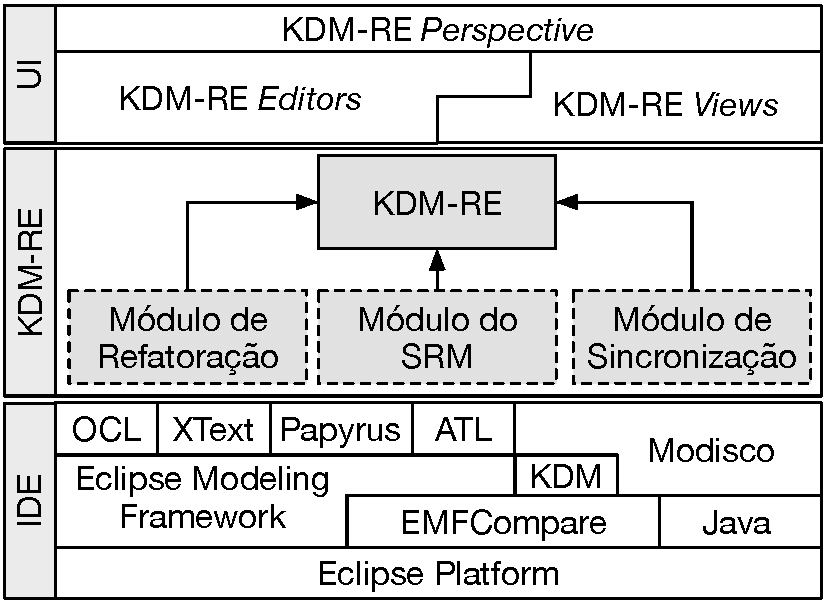
\includegraphics[scale=0.75]{images/arquitetura_KDM-RE}
	\fautor
\end{figure}

Na segunda camada é onde os módulos da KDM-RE são definidos. O módulo de refatoração utiliza EMF, ATL, OCL e MoDisco para criar um \textit{plug-in} onde o engenheiro de software pode aplicar refatorações em instâncias do metamodelo KDM. O módulo de sincronização utiliza o \textit{framework} EMFCompare e ATL. Por sua vez, o módulo do SRM utiliza EMF e XText. XText é utilizado no módulo do SRM para definir uma DSL para auxiliar a instanciação do metamodelo SRM. A última camada, UI, é responsável pela interface gráfica da ferramenta KDM-RE. Essa camada possui \textit{Wizards}, editores e visões para a aplicação, definição e reutilização das refatorações no contexto do KDM. Nas seções seguintes os três principais módulos da ferramenta KDM-RE são apresentados e discutidos.


\section{Módulo de Refatoração}\label{sec:modulo_de_refatoracao_kdm_re}

Nessa seção o módulo de refatoração é apresentado. Esse módulo foi implementado para prover suporte as refatorações criadas por meio das diretrizes apresentadas no Capítulo~\ref{chapter:catalogo_refactoring_KDM}. Na literatura é possível identificar um conjunto de técnicas e linguagens específicas para auxiliar a condução e especificação de transformação de modelos~\cite{Biehl_2010, Mens_2006, Allilaire_06}. Nesta Tese, a linguagem de transformação ATL~\cite{ATL_eclipse,Jouault_2008} foi escolhida para definir e aplicar refatorações no metamodelo KDM. Similarmente, as pre- e pós-condições foram implementadas em OCL. KDM-RE programaticamente executa as refatorações implementadas em ATL por meio da ATL EMF \textit{Transformation Virtual Machine}. As pre- e pós-condições são executadas na KDM-RE por meio da API Desden OCL\footnote{\texttt{http://www.dresden-ocl.org/}}. Essa API facilita a aplicação de OCL em qualquer metamodelo definido em EMF, no contexto desta Tese KDM. Como consequência, KDM-RE é capaz de suportar a detecção de violações semânticas estáticas em instâncias do metamodelo KDM.


Como já salientado no Capítulo~\ref{chapter:catalogo_refactoring_KDM} as refatorações foram definidas para serem executadas no contexto de instancias do metamodelo KDM. Dessa forma, é necessário primeiramente transformar um determinado sistema em instância do metamodelo KDM. Para tal, foi integrado a ferramenta MoDisco na KDM-RE como apresentado na Figura~\ref{fig:kdm_modisco_discovery}. Primeiramente, o engenheiro de software deve clicar com o botão direito em um projeto Java e escolher a opção \texttt{Knowledge Discovery} e em seguida escolher o menu \texttt{Discovery KDM MODEL}. MoDisco irá então transformar o código escrito na linguagem de programação Java para uma instancia do metamodelo KDM. 

\begin{figure}[h]
	\centering
	% Requires \usepackage{graphicx}
	\caption{KDM \textit{Discovery}.}
	\label{fig:kdm_modisco_discovery}
	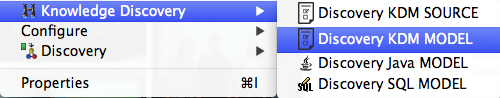
\includegraphics[scale=0.65]{images/kdm_discovery_kdm_re}
	\fautor
\end{figure}

Após a criação da instancia do metamodelo KDM o engenheiro de software pode aplicar as refatorações. A ferramenta KDM-RE permite que as refatorações sejam aplicadas por meio de duas interfaces gráficas. A primeira é uma extensão do editor gráfico da ferramenta MoDisco~\cite{Bruneliere_2014} que representa a instância do metamodelo em formato de árvore. A segunda interface gráfica é uma extensão do editor gráfico da ferramenta Papyrus\footnote{\texttt{https://eclipse.org/papyrus/}} que é uma ferramenta \sigla{CASE}{\textit{Computer-Aided Software Engineering}}. Por meio da segunda interface o engenheiro de software pode aplicar refatorações utilizando um diagrama de classe UML. Nota-se que nessa segunda interface de forma transparente as refatorações são de fato aplicadas em instâncias do KDM, o diagrama de classe UML é utilizado apenas como uma ponte entre as informações (nome de classe, atributos, métodos, etc) e as refatorações.

A primeira interface gráfica fornece uma visão de árvore da instância do metamodelo KDM (\textit{model browser}) como apresentado na Figura~\ref{fig:modisco_modeol_browser}. Lado esquerdo algumas das metaclasses (\texttt{ClassUnit}, \texttt{MethodUnit} e \texttt{StorableUnit}, etc) instanciadas do metamodelo KDM são apresentadas. Lado direito é onde as refatorações são aplicadas pelo engenheiro de software. Para aplicar as refatorações o engenheiro de software deve clicar com o botão direito em cima de uma determinada instância de metaclasse, por exemplo, \texttt{ClassUnit}, \texttt{MethodUnit}, \texttt{StorableUnit}, etc, assim, o menu \texttt{Refactoring KDM} irá aparecer como ilustrado na Figura~\ref{fig:kdm_re_refactoring_arvore}. Utilizando esse menu o engenheiro de software pode interagir com a instância do metamodelo KDM e escolher qual refatoração deve ser executada. Após o engenheiro de software clicar no menu \texttt{Refactoring KDM} e escolher uma determinada refatoração o processo se inicia. 

Para cada refatoração um determinado \textit{RefactoringWizard} é executado. Esse \textit{Wizard} irá guiar o engenheiro de software durante a aplicação da refatoração. Em cada refatoração a instância do metamodelo KDM deve ser analisada para identificar e obter os metadados das metaclasses que serão afetadas pela refatoração. Esses metadados são utilizadas tanto na ATL (refatoração) quanto na OCL (pré- e pós-condições). 


\begin{figure}[h]
	\centering
	% Requires \usepackage{graphicx}
	\caption{MoDisco \textit{Model Browser}.}
	\label{fig:modisco_modeol_browser}
	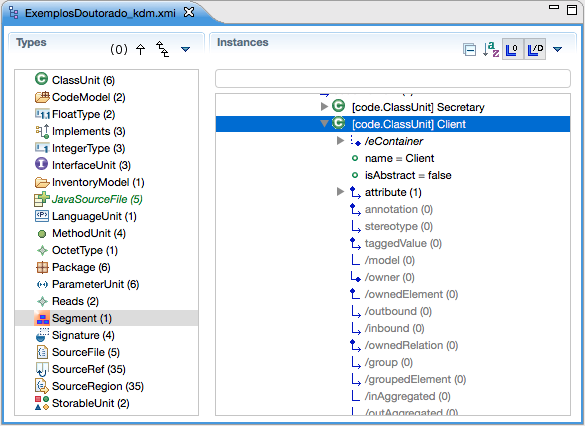
\includegraphics[scale=0.6]{images/kdm-re_modisco}
	\fautor
\end{figure}

\begin{figure}[h]
	\centering
	% Requires \usepackage{graphicx}
	\caption{KDM-RE \textit{Refactoring Browser}.}
	\label{fig:kdm_re_refactoring_arvore}
	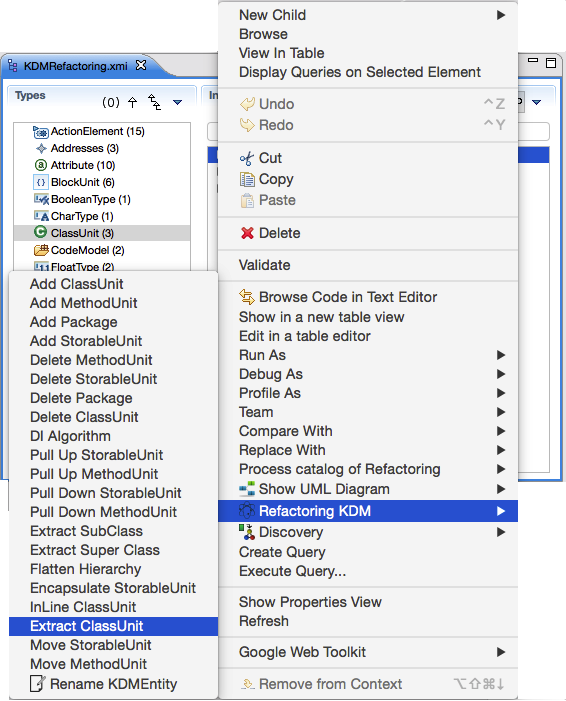
\includegraphics[scale=0.55]{images/novoMenuPopupKDM_RE}
	\fautor
\end{figure}


Por exemplo, suponha que o engenheiro de software identificou que uma instância da metaclasse \texttt{ClassUnit} está realizando o trabalho que deveria ser feita por duas instâncias (ver Figura~\ref{fig:kdm_re_wizard_extract_class}). Assim, o engenheiro de software deve aplicar a refatoração \texttt{Extract ClassUnit}. O primeiro passo é selecionar a instância da metaclasse \texttt{ClassUnit} para realizar a refatoração. Em seguida, deve-se selecionar a opção \texttt{Extract ClassUnit} no menu \texttt{Refactoring KDM}. Automaticamente KDM-RE irá criar um \textit{Wizard} para auxiliar o engenheiro de software como ilustrado na Figura~\ref{fig:kdm_re_wizard_extract_class}. Utilizando esse \textit{Wizard} o engenheiro de software define o nome da nova instância da metaclasse \texttt{ClassUnit}. Além disso, esse \textit{Wizard} permite visualizar todos as instâncias das metaclasses \texttt{StorableUnit} e \texttt{MethodUnit} que serão extraídas para a nova instância a ser criada. O \textit{Wizard} também permite especificar se instâncias da metaclasse \texttt{MethodUnit} devem ser criada para representar os métodos assessores (\textit{getters} e \textit{setters}). 

Uma característica importante da KDM-RE é a opção de visualizar previamente o resultado da refatoração. Assim, caso o engenheiro de software almejar visualizar o efeito da refatoração antes de efetivamente realiza-la o mesmo pode selecionar o botão \texttt{Preview}. Após clicar no botão \texttt{Preview} uma visão de comparação será criada como apresentado na Figura~\ref{fig:previa_resultado_extractClassUnit}. Essa visão de comparação contém duas principais partes. A parte superior representa quais instâncias foram deletadas, movidas e adicionadas de forma textual. Na parte inferior é possível visualizar graficamente a diferença entre as duas instâncias do metamodelo KDM, ou seja, a instância não refatorada (original) e a instância refatorada. O lado direito representa a instância do metamodelo KDM após a aplicação da refatoração \texttt{Extract ClassUnit} e o lado esquerdo representa a instância do metamodelo KDM antes da aplicação da refatoração. 

Como pode ser observado na Figura~\ref{fig:previa_resultado_extractClassUnit}, a instância direito do metamodelo KDM (instância refatorada) uma nova instância da metaclasse \texttt{ClassUnit} chamada \texttt{Document} foi criada - uma instância da metaclasse \texttt{StorableUnit} (\aspas{\texttt{CPF}}) foi movida para a nova \texttt{ClassUnit} \texttt{Document} - instâncias da metaclasse \texttt{MethodUnit} também foram criadas para representar os métodos assessores. A instância da metaclasse denominada \texttt{Pessoa} agora possui uma instância da metaclasse \texttt{StorableUnit} denominada \texttt{document} que representa um link entre as duas instâncias de \texttt{ClassUnit}.

\begin{figure}[h]
	\centering
	% Requires \usepackage{graphicx}
	\caption{\texttt{Extract ClassUnit} \textit{Wizard}.}
	\label{fig:kdm_re_wizard_extract_class}
	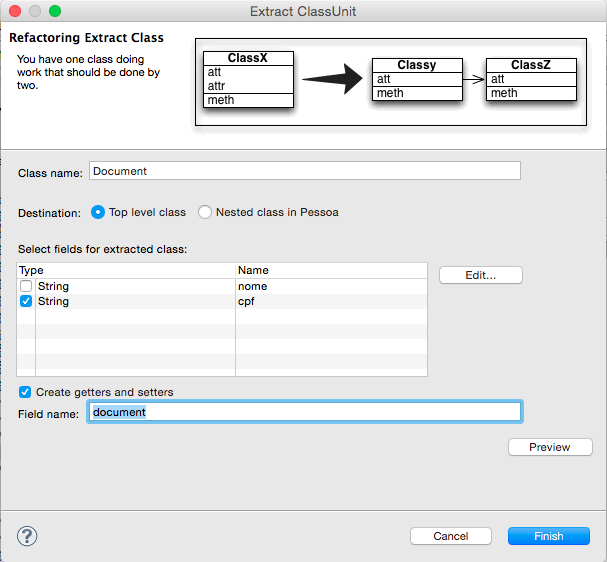
\includegraphics[scale=0.5]{images/extractClassEasierToExplainerEMFCOmpare}
	\fautor
\end{figure}

\begin{figure}[h]
	\centering
	% Requires \usepackage{graphicx}
	\caption{Prévia do resultado da refatoração \texttt{Extract ClassUnit}.}
	\label{fig:previa_resultado_extractClassUnit}
	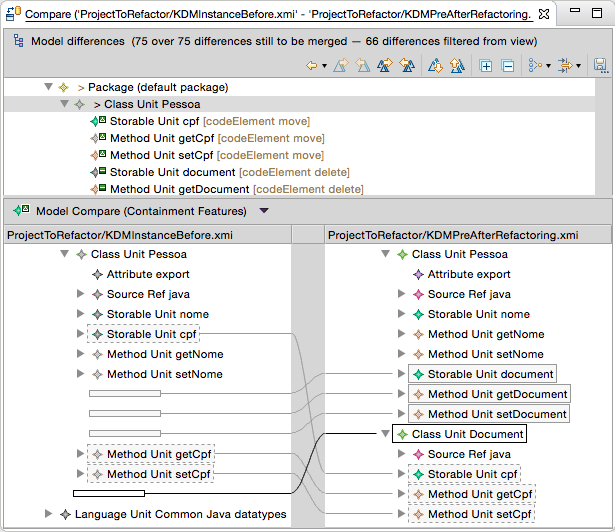
\includegraphics[scale=0.5]{images/previaRefatoracaoExtractClassUnitEMFCOmpare}
	\fautor
\end{figure}


Após especificar todas as entradas necessárias e visualizar o efeito que a refatoração irá resultar na instância do metamodelo KDM o engenheiro de software deve clicar no botão \textit{Finish}. A KDM-RE executa a API Dresden OCL para verificar as pré-condições. Caso as pré-condições forem satisfeitas a refatoração \texttt{Extract ClassUnit} é executada efetivamente. A execução da refatoração é totalmente realizada com base na ATL. As entradas informadas pelo engenheiro de software no \textit{Wizard} são enviadas para ATLs pré-definidas e em seguida são executadas programaticamente pela KDM-RE por meio da ATL EMF \textit{Transformation Virtual Machine}\footnote{\texttt{https://wiki.eclipse.org/ATL/EMFTVM}}. Em seguida, a KDM-RE  executa a API Dresden OCL para verificar as pós-condições. 


Embora a primeira interface gráfica seja útil para aplicar refatorações diretamente em instâncias do metamodelo KDM, a mesma não é intuitiva. Dessa forma, a segunda interface gráfica tem como objetivo deixar as refatorações mais fáceis e intuitivas de serem aplicadas. Por exemplo, embora~\citeonline{Fowler1999} tenha criado um catálogo de refatorações para ser utilizado em código-fonte, mais de 60\% das refatorações (44 de 72) são ilustradas utilizando modelos, mais especificadamente diagramas de classes da UML. Além disso, ~\citeonline{Zhang_2005, Boger_2003} afirmam que algumas refatorações, por exemplo, \texttt{Extract Method}, são mais naturais quando executadas diretamente no código-fonte. Enquanto que outras refatorações, como: \texttt{Rename Class}, \texttt{Pull Up Method}, \texttt{Push Down Method}, etc, podem ser aplicadas tanto em código-fonte quando em modelos; já as refatorações que lidam com herança, tais como \texttt{Extract Class}, \texttt{Extract Interface}, \texttt{Replace Inheritance with Delegation}, são mais intuitivas quando aplicadas diretamente em nível de modelo, tais como diagrama de classe da UML. 

Neste contexto, a KDM-RE foi integrada com a ferramenta CASE Papyrus para utilizar o diagrama de classe da UML. Para utilizar essa segunda interface primeiramente é necessário transformar a instância do metamodelo KDM para uma instância da UML. Assim, as refatorações definidas na KDM-RE podem ser aplicadas diretamente em diagramas da UML, por exemplo, pode-se aplicar refatorações por meio do diagrama de classe. É importante observar que embora as refatorações sejam aplicadas graficamente por meio do diagrama de classe da UML todas as refatorações (transformações) são aplicadas transparentemente na instância do metamodelo KDM e não na instância da UML - apenas informações são extraídas do diagrama de classe da UML e são enviados como entrada para as refatorações pré-definida em ATL. %Tecnicamente essa segunda interface é implementada como uma extensão da ferramenta CASE Papyrus.


Os passos para utilizar a segunda interface são similares a primeira interface. Porém, um passo a mais se faz necessário para utilizar a segunda interface. Deve-se gerar uma instância do metamodelo UML tendo como base uma instância do metamodelo KDM. A geração da instância do metamodelo UML é totalmente apoia por um \textit{plug-in} denominado \texttt{DiscoverUmlModelFromKdmModel} do MoDisco. Esse \textit{plug-in} utiliza regras ATL para criar uma instância do metamodelo UML tendo como base outra instância do metamodelo KDM. Por exemplo, na Figura~\ref{fig:kdmToUML} são apresentadas duas instâncias dos metamodelos UML (lado esquerdo) e KDM (lado direito) após a transformação, respectivamente.

\begin{figure}[!h]
	\centering
	% Requires \usepackage{graphicx}
	\caption{Instância UML gerada a partir do KDM.}
	\label{fig:kdmToUML}
	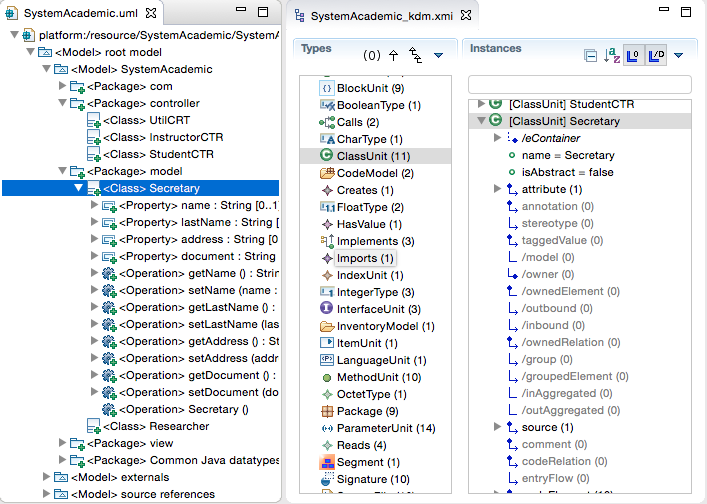
\includegraphics[scale=0.5]{images/kdmToUML}
	\fautor
\end{figure}

Após a criação da instância do metamodelo UML o próximo passo é utilizar a ferramenta CASE Papyrus para exibir a nova instância do metamodelo UML por meio do diagrama de classe como apresentado na Figura~\ref{fig:kdmToUML_diagrama_de_classe}. Por meio desse diagrama a KDM-RE permite que o engenheiro de software realize refatorações. Por exemplo, na Figura~\ref{fig:refatoracao_papyrus_KDM_iteragir} é ilustrado que primeiramente o engenheiro de software deve clicar com o botão direito em cima do elemento que almeja refatorar, nesse caso a classe \texttt{Secretary}, escolher a opção \texttt{Refactoring Model} e em seguida decidir qual refatoração aplicar, nesse exemplo - \texttt{Extract ClassUnit}. Em seguida um \textit{RefactoringWizard} similar ao apresentado na Figura~\ref{fig:kdm_re_wizard_extract_class} é executado. O mesmo também irá guiar o engenheiro de software durante a aplicação da refatoração. Da mesma forma como na primeira interface, na segunda interface o engenheiro de software pode solicitar também a realização de uma prévia da refatoração. O resultado dessa solicitação será uma interface similar a apresentada na Figura~\ref{fig:previa_resultado_extractClassUnit}.

\begin{figure}[!h]
	\centering
	% Requires \usepackage{graphicx}
	\caption{Diagrama de Classe da UML gerada a partir do KDM.}
	\label{fig:kdmToUML_diagrama_de_classe}
	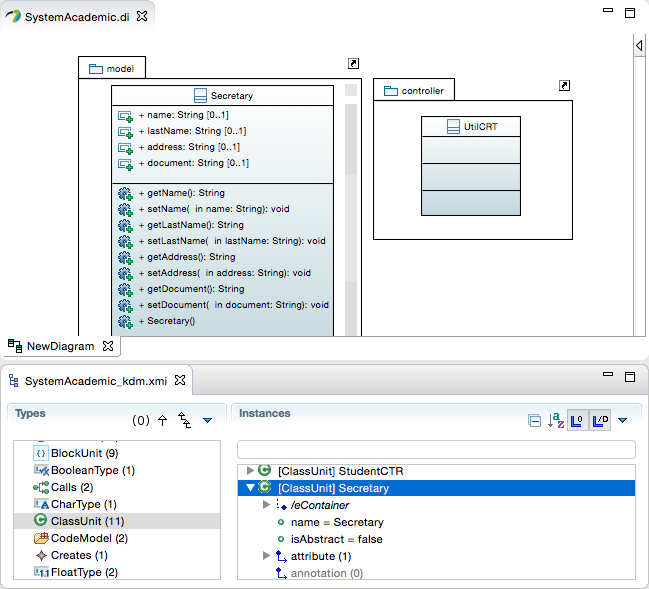
\includegraphics[scale=0.5]{images/refatoracao_UML_papyrus}
	\fautor
\end{figure}

As informações fornecidas pelo engenheiro de software no \textit{Wizard} são enviadas para ATLs pré-definidas e em seguida são executadas programaticamente pela KDM-RE por meio da ATL EMF \textit{Transformation Virtual Machine}. O resultado da refatoração altera a instância do metamodelo KDM e é replicado automaticamente no diagrama de classe da UML, portanto, o engenheiro de software pode visualizar graficamente no diagrama de classe UML o resultado da refatoração.

\begin{figure}[!h]
	\centering
	% Requires \usepackage{graphicx}
	\caption{Refatorações por meio do Diagrama de Classe.}
	\label{fig:refatoracao_papyrus_KDM_iteragir}
	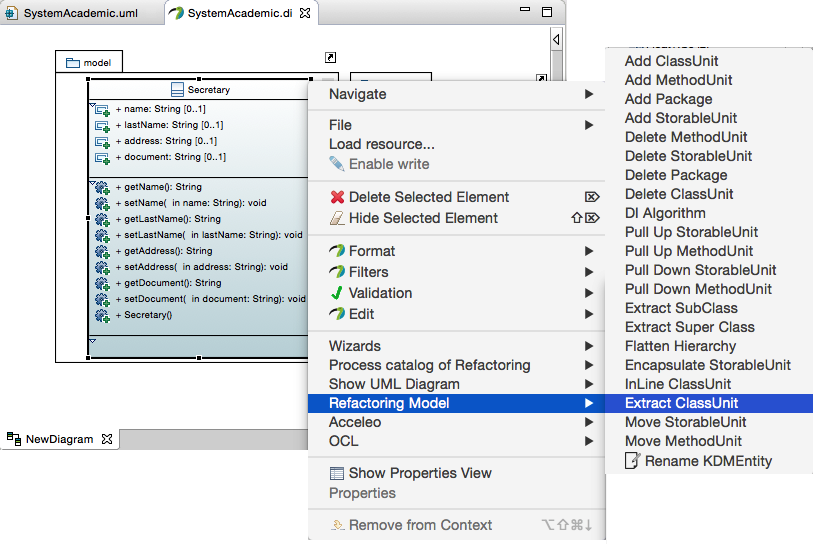
\includegraphics[scale=0.5]{images/kdm_uml_papyrus_refactoring_extract_class_new}
	\fautor
\end{figure}

\section{Módulo do SRM}\label{label:sec_modulo_do_srm}

Nessa seção é apresentado um módulo desenvolvido para fornecer suporte ao metamodelo SRM apresentado no Capítulo~\ref{chapter:Toward_a_Refactoring_Metamodel_for_KDM}  Figura~\ref{fig:meta_modelo_SRM}. Esse módulo implementa o metamodelo SRM utilizando EMF por meio do meta-metamodelo Ecore. Nesse módulo também foi definido uma linguagens específica de domínio (DSL) para facilitar a instanciação do metamodelo SRM. A gramática dessa DSL é apresentada no Capítulo~\ref{chapter:Toward_a_Refactoring_Metamodel_for_KDM}, mais detalhadamente nos Códigos-fontes~\ref{lst:dsl_part_1}, \ref{lst:dsl_part_2}, \ref{lst:dsl_part_3}, \ref{lst:dsl_part_4} e \ref{lst:dsl_part_5}.


Esse módulo fornece uma forma de compartilhar e reutilizar refatorações por meio de instâncias do metamodelo SRM. Para permitir o reúso e compartilhamento de refatorações um repositório remoto foi criado. Esse repositório remoto é dedicado para executar solicitações RESTful. Instâncias do metamodelo SRM são enviadas e recebidas por meio da API RESTful. Isso é possível pois as instâncias do SRM são arquivos que persistidos no formato XMI. \sigla{JPA}{Java Persistence API} e o banco de dados MySQL foram utilizados para realizar as persistências das instâncias do metamodelo SRM.

%Para utilizar as vantagens dos metamodelo SRM, os engenheiros de modernização precisam ter conhecimento de linguagem de programação avançada. Eles devem estar familiarizados como as semânticas das refatorações (por exemplo, qual(is) é (são) o(s) pré-requisito(s) para a execução de uma refatoração) e como/onde utilizar e programar tais refatorações. Além disso, a instanciação de uma refatoração utilizando o metamodelo SRM é bastante verbosa, complexa e propensa a erros, pois exige conhecimento avançadas de refatoração e habilidades de programação em relação a API Ecore/EMF. Como salientado no Capítulo~\ref{chapter:Toward_a_Refactoring_Metamodel_for_KDM} o metamodelo SRM foi desenvolvido para permitir a reutilização de metaclasses já definidas no metamodelo KDM. Mais especificadamente os elementos estruturais que são utilizados em uma refatoração são representados por metaclasses previamente já definidas no metamodelo KDM, tais como: \texttt{ClassUnit}, \texttt{InterfaceUnit}, \texttt{Package}, \texttt{StorableUnit}, etc.

%No Código-fonte~\ref{cod:instancia_do_SRM} é apresentado um trecho onde é feita a instanciação em memória de algumas metaclasses definidas no metamodelo SRM. Note que nesse código-fonte a instanciação das metaclasses do metamodelo SRM é um processo verboso e propenso a erros. Para instanciar o metamodelo SRM o engenheiro deve saber utilizar a API do \textit{framework} EMF. Metaclasses são instanciadas em EMF utilizando o conceito de fabrica (em inglês - \textit{Factory}). Cada fabrica de uma metaclasse possui um método \texttt{createX}, onde X representa o nome da metaclasse do metamodelo. Para criar uma instancia válida do metamodelo SRM o engenheiro de modernização deve seguir um conjunto de passos. Por exemplo, como pode ser observado na linha 1 do Código-fonte~\ref{cod:instancia_do_SRM} uma instância da metaclasse \texttt{Author} é criada por meio da interface \texttt{RefactoringModelFactory} e do método \texttt{createAuthor()}. Em seguida, todos os meta-atributos da metaclasse \texttt{Author} devem ser especificados como apresentado nas linhas 2 e 3 do Código-fonte~\ref{cod:instancia_do_SRM}. Nas linhas 4-14 outras metaclasses do metamodelo SRM são instanciadas. 


%Como apresentado e salientado no Capítulo~\ref{chapter:Toward_a_Refactoring_Metamodel_for_KDM} a instanciação de uma refatoração por meio do SRM pode ser um processo demorado e suscetível a erro. Para diminuir a quantidade de código-fonte, esforço obrigatórios e competência necessárias para instanciar refatorações utilizando o metamodelo SRM, a KDM-RE provê uma DSL que auxilia a instanciação de refatorações sistematicamente. Na parte superior a esquerda da Figura~\ref{fig:DSL_SRM} é possível visualizar o relacionamento entre a DSL criada e as metaclasses do metamodelo SRM. 

Por meio das gramáticas apresentadas nos Códigos-fontes~\ref{lst:dsl_part_1}, \ref{lst:dsl_part_2}, \ref{lst:dsl_part_3}, \ref{lst:dsl_part_4} e \ref{lst:dsl_part_5} Xtext gera um editor textual para o ambiente de desenvolvimento Eclipse IDE. Esse editor textual provê \textit{highlighting} de sintaxe, \textit{autocomplete} de código e navegação de código. Na parte superior a esquerda da Figura~\ref{fig:DSL_SRM} é possível visualizar trechos da DSL resultante. Além disso, essa figura ilustra o relacionamento entre a DSL criada e as metaclasses do metamodelo SRM, ou seja, representa que a sintaxe da DSL esta em conformidade com as metaclasses do SRM.

%\begin{codigo}[caption={[Instanciação do metamodelo SRM programaticamente.] Instanciação do metamodelo SRM.},escapeinside={(*@}{@*)}, basicstyle=\footnotesize, label={cod:instancia_do_SRM}, language=Java]{Name}
%Author author = RefactoringModelFactory.eINSTANCE.createAuthor();
%author.setName("Rafael");
%author.setLastName("Durelli");
%RefactoringModel rM = RefactoringModelFactory.eINSTANCE.createRefactoringModel();
%rM.setAuthor(author);
%RefactoringLibrary library = RefactoringModelFactory.eINSTANCE.createRefactoringLibrary();
%lib.setName("Fowler's refactorings");
%lib.setDescription("Contains some Fowler's refactorings such as ExtractClass, RenameElements, PushMethod, PushAttribute, etc.");
%lib.setShortDescription("Fine grained Refactorings");
%rM.getLibraries().add(lib);
%Catalog cat = RefactoringModelFactory.eINSTANCE.createCatalog();
%cat.setAuthor(author);
%cat.setName("Fowler's catalog");
%libr.getCatalogs().add(cat);
%...
%\end{codigo}

\begin{figure}[!h]
	\centering
	% Requires \usepackage{graphicx}
	\caption{DSL para auxiliar a instanciação do SRM.}
	\label{fig:DSL_SRM}
	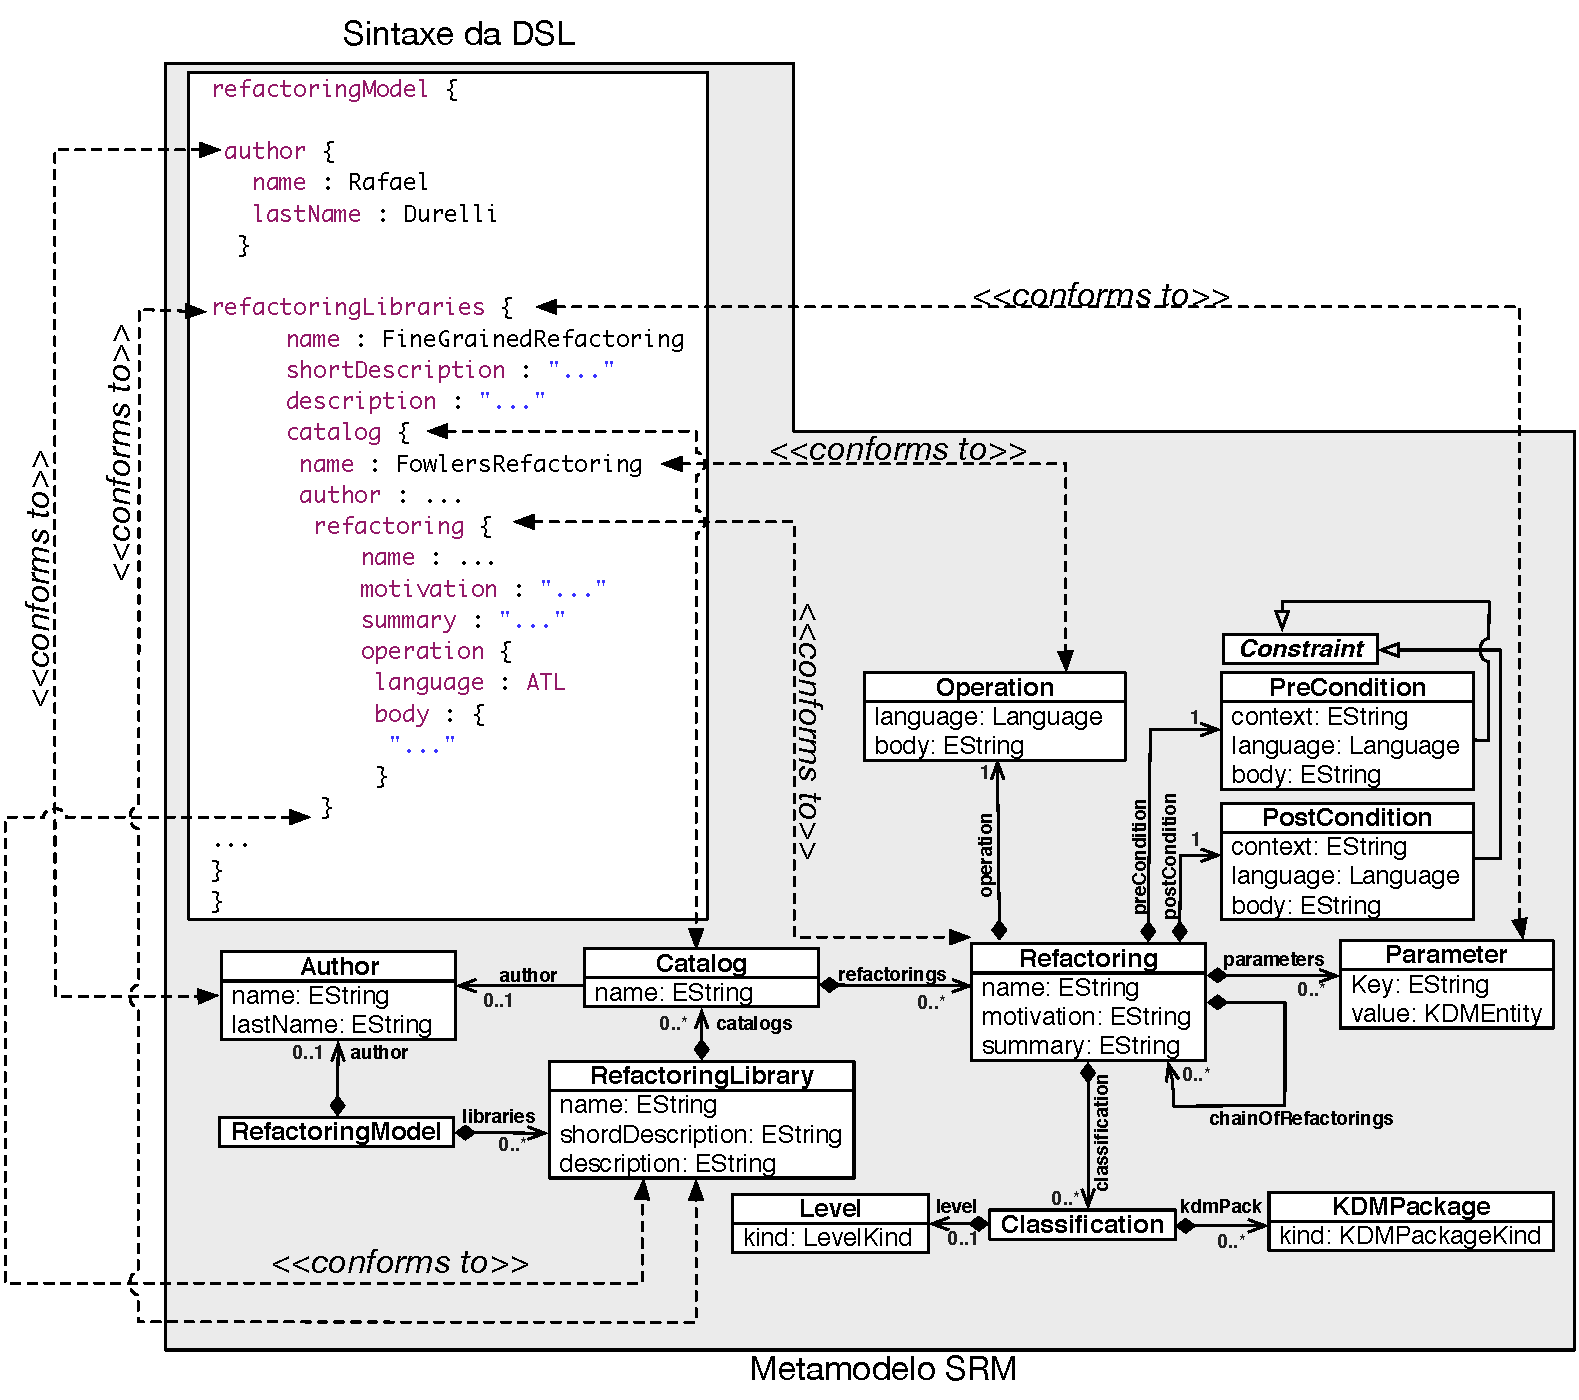
\includegraphics[scale=0.6]{images/MetaModelEDSL2}
	\fautor
\end{figure}

Cada trecho de código da DSL representa uma instancia de uma metaclasse do metamodelo SRM, ou seja, cada declaração da DSL está em conformidade com uma metaclasse do SRM. Por exemplo, a palavra-chave \texttt{refactoringModel} \texttt{author} entre \aspas{\{} e \aspas{\}} representa a instanciação da metaclasse \texttt{Author} do SRM que possui dois meta-atributos: \texttt{name} e \texttt{lastName}. A DSL criada para auxiliar a instanciação do SRM foi desenvolvida utilizando Xtext\footnote{\texttt{https://www.eclipse.org/Xtext/}}. Xtext é um \textit{framework} do Eclipse\footnote{\texttt{https://www.eclipse.org}} que facilita a definição de gramática\footnote{Gramáticas representam a definição formal de um sintaxe textual concreta. Consistem em um conjunto de regras de produção para definir como o \textit{textual input} (ou seja, sentenças) são representadas. Basicamente, as regras de produção podem ser representadas utilizando \sigla{BNF}{\textit{Backus–Naur Form}}, por exemplo, \textit{S ::= P1 ... Pn}, essa gramática define um símbolo \textit{S} por um conjunto de expressões \textit{P1 ... Pn}.} 
com a utilização de um metamodelo que foi definido utilizando EMF. Xtext tem como principal objetivo automatizar e agilizar o processo de desenvolvimento de DSLs. Note que a sintaxe da DSL segue as terminologias e conceitos definidos no metamodelo SRM para facilitar a utilização da DSL e o entendimento do metamodelo SRM.

%Em Xtext a gramática segue uma notação similar ao \textit{Backus–Naur Form} (BNF) chamada de regras do \textit{parser}. Tais regras representam a sintaxe concreta da DSL. Note que para facilitar o entendimento da DSL, trechos da mesma são mostradas em listagens de códigos separados, bem como símbolos para explanar o propósito de uma terminada linha da gramática. No Código-fonte~\ref{lst:dsl_part_1} é ilustrado o primeiro trecho da gramática concreta da DSL desenvolvida. A gramática começa com a definição do nome da DSL (SRM) (ver Código-fonte~\ref{lst:dsl_part_1} \ding{182}). Em sequência é definido os metamodelos que devem ser importados para serem utilizados durante a criação da DSL: o metamodelo SRM\ding{183} e o Ecore\ding{184}.


%\begin{lstlisting}[language=Xtext, frame=single, basicstyle={\scriptsize}, mathescape=true, label={lst:dsl_part_1}, caption={Gramática da DSL - parte 1}]
%$\textrm{\ding{182}}$ grammar refactoring.xtext.SRM with org.eclipse.xtext.common.Terminals 
%$\textrm{\ding{183}}$ import platform:/resource/refactoring/model/SRM.ecore
%$\textrm{\ding{184}}$ import http://www.eclipse.org/emf/2002/Ecore as ecore
%RefactoringModel: 
%	$\textrm{\ding{185}}$ `refactoringModel' name = ID `{'
%	$\textrm{\ding{186}}$ author = Author
%	$\textrm{\ding{187}}$ libraries += RefactoringLibrary$^{*}$;
%	`}'
%\end{lstlisting}


%Em seguida é criado a primeira regra. Essa regra começa com a definição da metaclasse \texttt{RefactoringModel}. O corpo da regra começa logo após os \aspas{\texttt{:}}. Primeiramente para o entendimento da regra, é importante destacar que literais de \textit{string} (em Xtext os literais podem ser expressos com aspas simples ou duplas) definem palavras-chave da DSL. Como pode ser observado no Código-fonte~\ref{lst:dsl_part_1} é esperado a palavra-chave \texttt{refactoringModel}\ding{185} seguido por um \texttt{ID} e \aspas{\{}. A gramática que rege o objeto \texttt{ID} é definida como uma sequência ilimitada de maiúsculas e minúsculas, números e o carácter de sublinhado, embora possa não começa por um dígito. A gramática que representa o nó \texttt{ID}\ding{182} pode ser visualizada no Código-fonte~\ref{lst:dsl_part_2}. 

%\begin{lstlisting}[language=Xtext, frame=single, basicstyle=\scriptsize, mathescape=true, label={lst:dsl_part_2}, caption={Gramática da DSL - parte 2}]
%	$\textrm{\ding{182}}$ terminal ID: (`a'..`z' | `A'..`Z'|`_')(`a'..`z' | `A'..`Z'|`_'|`0'..`9')*;
%\end{lstlisting}

%Ainda no Código-fonte~\ref{lst:dsl_part_1} a expressão \texttt{author=Author}\ding{186} especifica que pode-se instanciar uma instancia da metaclasse \texttt{Author}. A expressão \texttt{(libraries += RefactoringLibrary)$^{*}$}\ding{187} descrita no Código-fonte~\ref{lst:dsl_part_1} especifica que pode-se instanciar várias instâncias da metaclasse \texttt{RefactoringLibrary}. O operador estrela, \aspas{\texttt{*}}, ilustra que o número de elementos (nesse caso \texttt{RefactoringLibrary}) é arbitrário; em particular, ele pode ser qualquer número \texttt{>=} 0. Operador \texttt{+=} por sua vez representa que a propriedade \texttt{libraries} será uma lista do tipo \texttt{RefactoringLibrary}.

%\begin{lstlisting}[language=Xtext, frame=single, basicstyle=\scriptsize, mathescape=true, label={lst:dsl_part_3}, caption={Gramática da DSL - parte 3}]
%Author:
%	$\textrm{\ding{182}}$ `author' `{'
%	$\textrm{\ding{183}}$ `name' `:' name = ID  
%		$\textrm{\ding{229} \ding{184}}$ `lastName' `:' lastName = ID; 
%`}'
%RefactoringLibrary:
%	$\textrm{\ding{185}}$ `refactoringLibraries' `{'
%	$\textrm{\ding{186}}$ `name' `:' name = ID  
%		$\textrm{\ding{229}}$ `shortDescription' `:' shortDescription = STRING
%		$\textrm{\ding{229}}$ `description' `:' description = STRING
%		$\textrm{\ding{229}}$ $\textrm{\ding{187}}$ catalogs += Catalog$^{*}$
%`}'
%\end{lstlisting}

%A definição das regras que regem as metaclasses \texttt{Author} e \texttt{RefactoringLibrary} são apresentadas no Código-fonte~\ref{lst:dsl_part_3}. A regra para a definição de \texttt{Author} começa com a definição da palavra-chave \texttt{author} seguida por um \aspas{\{}\ding{182}. Em seguida a palavra-chave \texttt{name} é esperada, seguido por \aspas{\texttt{:}} \ding{183}. Posteriormente a palavra-chave \texttt{lastName} também é esperada, seguido por \aspas{\texttt{:}} \ding{184}. Na linha 6 do Código-fonte~\ref{lst:dsl_part_3} começa a definição da regra da metaclasse \texttt{RefactoringLibrary}. A regra para a definição de \texttt{RefactoringLibrary} começa com a definição da palavra-chave \texttt{refactoringLibraries} seguida por um \aspas{\{}\ding{185}. Em seguida, deve-se especificar a palavra-chave \texttt{name} e \texttt{:}. Posteriormente, as palavras-chaves \texttt{shortDescription} e \texttt{description} são especificadas nas linhas 9 e 10, respectivamente. A expressão descrita na Linha 11 representa que pode haver qualquer número de instâncias da metaclasse \texttt{Catalog}.

%\begin{lstlisting}[language=Xtext, frame=single, basicstyle=\scriptsize, mathescape=true, label={lst:dsl_part_4}, caption={Gramática da DSL - parte 4}]
%Catalog:
%	$\textrm{\ding{182}}$`catalog' `{' 
%		$\textrm{\ding{229} \ding{183}}$`name' `:' name=ID
%		$\textrm{\ding{229} \ding{184}}$`author' `:' author=[Author]
%		$\textrm{\ding{229} \ding{185}}$refactorings += Refactoring$^{*}$
%	`}'
%Refactoring:
%	`refactoring' `{' 
%		$\textrm{\ding{229}}$`name' `:' name = ID
%		$\textrm{\ding{229}}$`motivation' `:' motivation = STRING
%		$\textrm{\ding{229}}$`summary' `:' summary = STRING
%		$\textrm{\ding{229} \ding{186}}$ operation = Operation?
%		$\textrm{\ding{229} \ding{187}}$ preCondition = PreCondition?
%		$\textrm{\ding{229} \ding{188}}$ postCondition = PostCondition?
%		$\textrm{\ding{229} \ding{189}}$ classification = Classification
%		$\textrm{\ding{229} \ding{190}}$(`containedRefactoring' `:' chainOfRefactoring+=Refactoring)$^{*}$
%	`}'
%\end{lstlisting}

%O Código-fonte~\ref{lst:dsl_part_4} representa as sintaxes concretas das metaclasses \texttt{Catalog} e \texttt{Refactoring}. A sintaxe concreta da metaclasse \texttt{Catalog} começa com a palavra-chave \texttt{catalog} seguida por um \aspas{\{}\ding{182}. Em seguida o nome do catálogo de refatoração deve ser especifica por meio da palavra-chave \texttt{name} \ding{183}. Posteriormente, deve-se especificar uma instância da metaclasse \texttt{Author}, informando quem é o autor desse catalogo de refatoração, ver Código-fonte~\ref{lst:dsl_part_4}\ding{184}. Na Linha 5 do Código-fonte~\ref{lst:dsl_part_4} deve-se informar várias instâncias da metaclasse \texttt{Refactoring}, essa sintaxe representa as refatorações que compõem esse catalogo de refatoração. Nas linhas 7-16 a definição da sintaxe concreta para a definição de uma refatoração por meio do metamodelo SRM é apresentada. Inicialmente, uma refatoração deve possuir um nome, conforme ilustrado na linha 9 do Código-fonte~\ref{lst:dsl_part_4}. Posteriormente, a motivação, bem como o resumo da refatoração também devem ser especificados, conforme apresentado nas linhas 10 e 11 do Código-fonte~\ref{lst:dsl_part_4}. As linhas 12, 13, 14 e 15 informam que uma metaclasse do tipo \texttt{Operation}\ding{186}, \texttt{PreCondition}\ding{187}, \texttt{PostCondition}\ding{188} e \texttt{Classification} \ding{189} devem ser instanciadas, respectivamente. Na linha 16 representa a sintaxe da DSL para especificar um conjunto de refatorações que quando combinadas podem realizar refatorações complexas.

%\begin{lstlisting}[language=Xtext, frame=single, basicstyle=\scriptsize, mathescape=true, label={lst:dsl_part_5}, caption={Gramática da DSL - parte 5}]
%Operation: 
%	$\textrm{\ding{182}}$`operation' `{'
%		$\textrm{\ding{229}}$`language' `:' language=Language
%		`body' `:' `{'
%			$\textrm{\ding{229} \ding{184}}$body = STRING
%		`}'
%	`}'
%PreCondition: 
%	$\textrm{\ding{185}}$`preCondition' `{'
%		$\textrm{\ding{229}}$`context' `:' context=STRING
%		$\textrm{\ding{229}}$`language' `:' language=Language
%		`body' `:' `{' 
%			$\textrm{\ding{229}}$body=STRING	
%		`}'
%	`}'
%PostCondition: 
%	$\textrm{\ding{186}}$`postCondition' `{'
%		$\textrm{\ding{229}}$`context' `:' context=STRING
%		$\textrm{\ding{229}}$`language' `:' language=Language
%		`body' `:' `{' 
%			$\textrm{\ding{229}}$body=STRING	
%		`}'
%	`}'
%enum Language: 
%	ATL | OCL | XQuery
%\end{lstlisting}

\begin{figure}[!h]
	\centering
	% Requires \usepackage{graphicx}
	\caption{Instanciando a DSL.}
	\label{fig:creatingSRMDSL}
	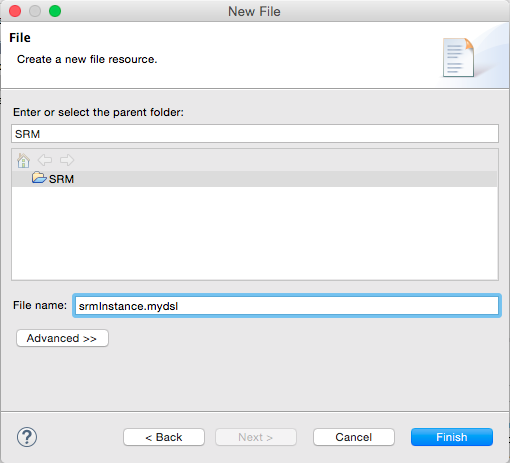
\includegraphics[scale=0.7]{images/creatingSRMDSL}
	\fautor
\end{figure}


\begin{figure}[!h]
	\centering
	% Requires \usepackage{graphicx}
	\caption{Editor Textual para instanciar o metamodelo SRM.}
	\label{fig:editor_SRM_metamodel_ECORE}
	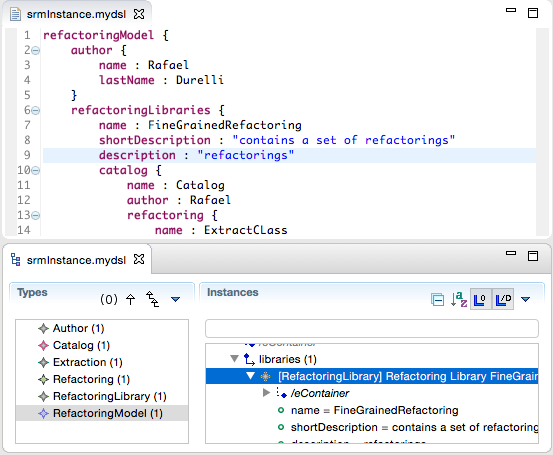
\includegraphics[scale=0.65]{images/dsl_SRM_ECORE}
	\fautor
\end{figure}

\begin{figure}[!h]
	\centering
	% Requires \usepackage{graphicx}
	\caption{Menu para enviar instâncias do metamodelo SRM.}
	\label{fig:editor_SRM_metamodel_ECORE_menu}
	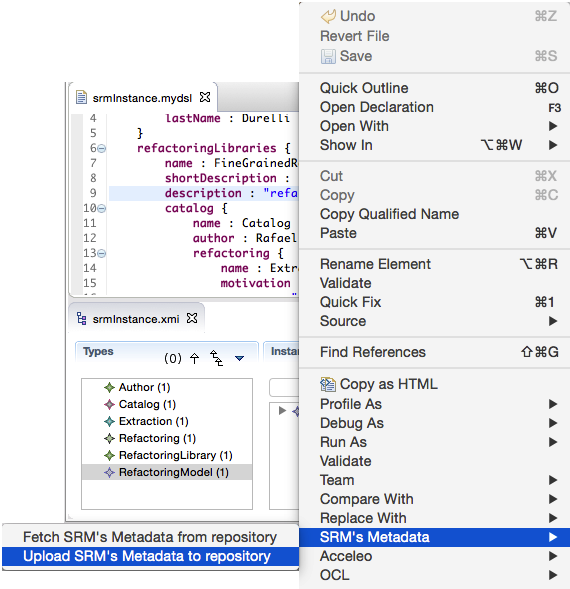
\includegraphics[scale=0.65]{images/SRM_Upload_Image}
	\fautor
\end{figure}

%No Código-fonte~\ref{lst:dsl_part_5} as sintaxes concretas das metaclasses \texttt{Operation}, \texttt{PreCondition} e \texttt{PostCondition} são definidas. A sintaxe concreta da metaclasse \texttt{Operation} inicia com a palavra-chave \texttt{operation} seguida por um \aspas{\{}\ding{182}. Em seguida, deve-se especificar qual a linguagem que a operação/refatoração será escrita. \texttt{Language} é uma enumeração (\textit{enum}) que está representado na linha 24 do Código-fonte~\ref{lst:dsl_part_5}. A linha 5 representa a sintaxe concreta para especificar o \aspas{corpo} da operação/refatoração propriamente dita \ding{184}. Na linha 8 a sintaxe concreta da metaclasse \texttt{PreCondition} é definida. A sintaxe concreta inicia com a palavra-chave \texttt{preCondition} seguida por um \aspas{\{}\ding{182}, \texttt{context}, \texttt{language} e \texttt{body}. A sintaxe concreta da metaclasse \texttt{PostCondition} é definida nas linhas 16 até 23. Note que a sintaxe é similar à sintaxe definida na metaclasse \texttt{PreCondition}. A partir das gramáticas da DSL apresentadas XText gera um editor textual no ambiente de desenvolvimento Eclipse IDE. Esse editor provê para a KDM-RE \textit{highlighting} de sintaxe, \textit{code completion} e \textit{code navigation}. O editor resultante pode ser observado na Figura~\ref{fig:editor_SRM_metamodel_ECORE}.


%Identificar e reutilizar artefatos em nível de modelos é uma limitação hoje em dia~\cite{Rocco_2015}. Essa limitação faz com que modernizadores geralmente tenham que recriar soluções já existentes, tais como: metamodelos, transformações, etc, diminuindo assim a produtividade e benefícios defendidos pelo MDE. Dessa forma, para facilitar e promover o compartilhamento e o reúso de refatorações por meio do metamodelo SRM é necessário uma forma que permita que modernizadores possam enviar, analisar e reutilizar as refatorações instanciadas para um artefato central. Assim, outros modernizadores podem contribuir com a criação de um conjunto de metadados sobre refatorações para que outros modernizadores possam pesquisar, identificar e reutilizar refatorações em seu projeto durante a modernização. 

%Neste contexto, um repositório foi criado para persistir instâncias do metamodelo SRM, onde tais instâncias representam metadados sobre refatorações que podem ser pesquisas e reutilizadas por outros modernizadores. Na Figura~\ref{fig:repositorio} é apresentado o diagrama de entidade e relacionamento do repositório. É importante observar que cada tabela apresentado nessa figura representa uma metaclasse do metamodelo SRM. Por exemplo, a metaclasse \texttt{Refactoring} apresentada na Figura~\ref{fig:meta_modelo_SRM} equivale a entidade \texttt{Refactoring} ilustrada na Figura~\ref{fig:repositorio}. 

%\begin{figure}[!h]
%	\centering
%	\caption{Diagrama de Entidade e Relacionamento do Metamodelo SRM.}
%	\label{fig:repositorio}
%	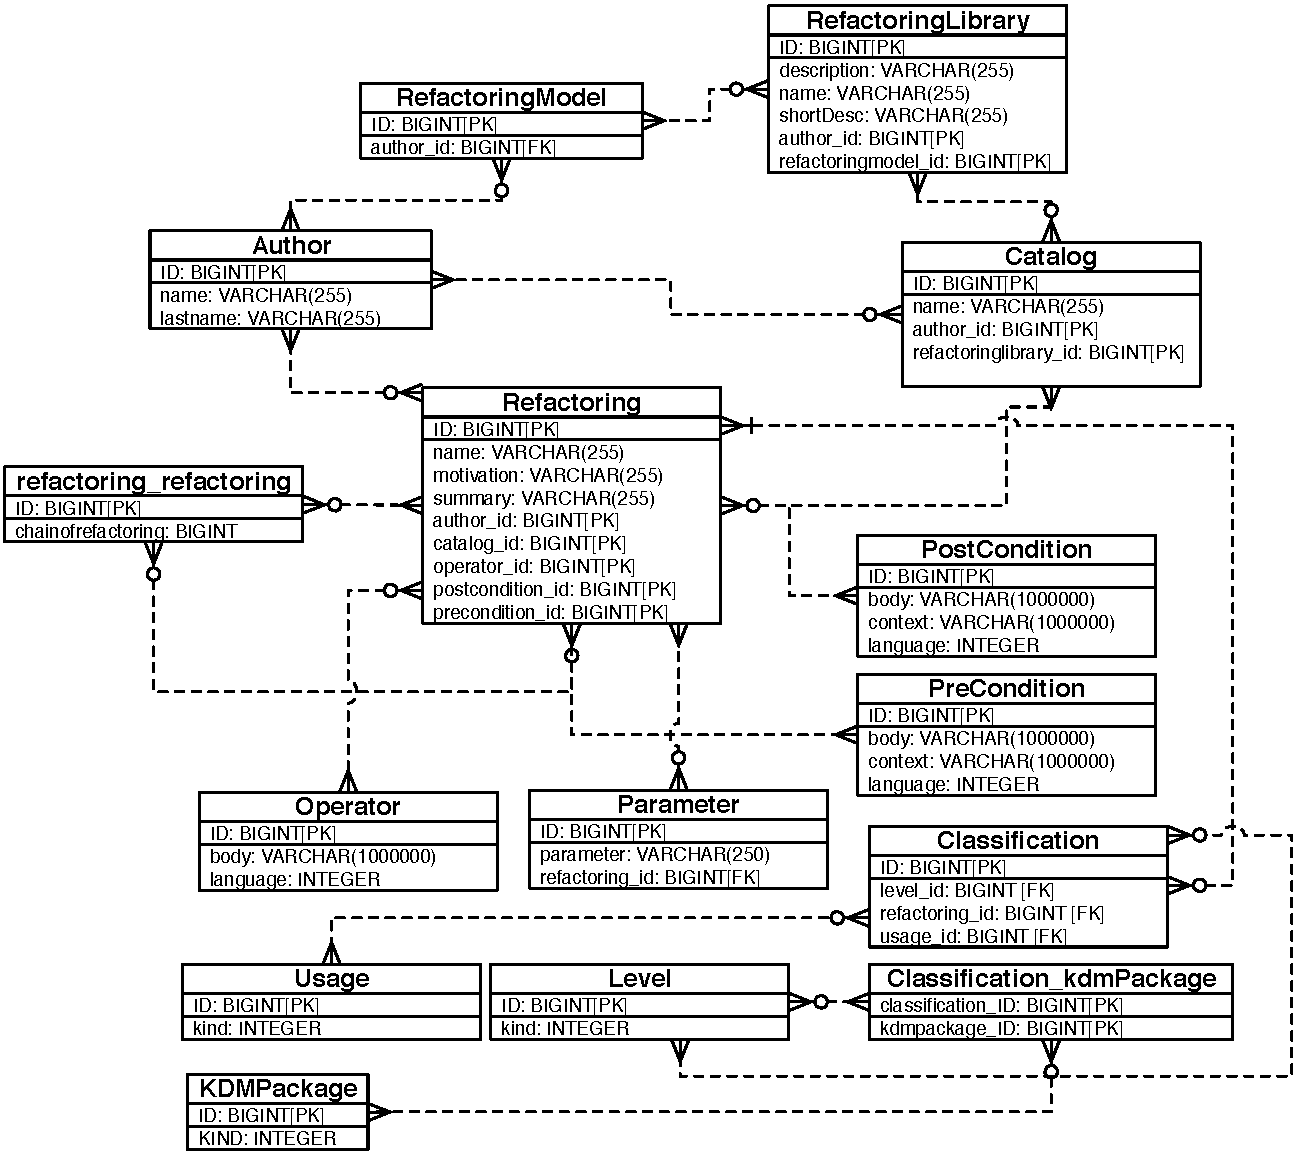
\includegraphics[scale=0.5]{images/ERD_refactoring}
%	\fautor
%\end{figure}

Para utilizar a DSL primeiramente o engenheiro de modernização precisa criar um arquivo com a extensão \aspas{.mydsl}. A KDM-RE fornece um \textit{wizard} para criar esse arquivo como apresentado na Figura~\ref{fig:creatingSRMDSL}. Por meio desse \textit{wizard} o engenheiro de modernização deve especificar um nome para o arquivo e também deve especificar a extensão do arquivo como \aspas{.mydsl}. É importante que o engenheiro de modernização especifique a extensão correta do arquivo, ou seja, \aspas{.mydsl}. Essa extensão é utilizada para o módulo do SRM identificar que o arquivo criado é na verdade a DSL definida na gramática apresentada nos Códigos-fontes~\ref{lst:dsl_part_1} -~\ref{lst:dsl_part_5}. No exemplo apresentado na Figura~\ref{fig:creatingSRMDSL} o arquivo foi definido como \texttt{srmInstance.mydsl}. Dessa forma, a KDM-RE automaticamente irá criar um editor para auxiliar o engenheiro de modernização a especificar uma refatoração utilizando as sintaxes da DSL. Após a criação do arquivo \texttt{srmInstance.mydsl} o engenheiro de modernização deve começar a especificar uma determinada refatoração como apresentado na Figura~\ref{fig:editor_SRM_metamodel_ECORE}. 


Adicionalmente, a KDM-RE fornece uma maneira de armazenar e compartilhar instâncias do metamodelo SRM. O principal objetivo é fazer com que refatorações definidas utilizando o metamodelo SRM sejam reutilizadas em projetos que utilizam o metamodelo KDM. Assim, após definir uma instância do metamodelo SRM utilizando a DSL, por meio do editor apresentado na Figura~\ref{fig:editor_SRM_metamodel_ECORE}, o engenheiro de modernização deve enviar os metadados de uma determinada instância do SRM para um repositório remoto. Esse processo é realizado por meio de um menu denominado \texttt{Upload SRM's Metadata to repository} - para interagir com esse menu o engenheiro deve clicar com o botão direito no editor textual da DSL e escolher \texttt{SRM's Metadata} como apresentado na Figura~\ref{fig:editor_SRM_metamodel_ECORE_menu}. Transparentemente a KDM-RE irá converter a sintaxe e a semântica da DSL em um arquivo XMI como ilustrado no Código-fonte~\ref{lst:xml_srm_convertido}. Note que nesse código-fonte os códigos em ATL e OCL (que representam a refatoração e as pré- e pós-condições) foram omitidos para facilitar o entendimento do arquivo XMI. 

Cada marcação apresentada nesse XMI representa uma metaclasse do metamodelo SRM. Por exemplo, \aspas{\textbf{<refactoringModel>}}, \aspas{\textbf{<libraries>}}, \aspas{\textbf{<catalogs>}} e \aspas{\textbf{<refactorings>}} estão em conformidades com as metaclasses \texttt{RefactoringModel}, \texttt{RefactoringLibrary}, \texttt{Catalog} e \texttt{Refactoring} do SRM, respectivamente. Adicionalmente, cada marcação contêm atributos que representam os meta-atributos de cada metaclasse do SRM.

\begin{lstlisting}[language=XML, frame=single, basicstyle={\scriptsize}, mathescape=true, label={lst:xml_srm_convertido}, caption={Arquivo XMI representando a instância do SRM.}]
<?xml version="1.0" encoding="ASCII"?>
<refactoringModel:RefactoringModel xmi:version="2.0" xmlns:xmi="http://www.omg.org/XMI" xmlns:xsi="http://www.w3.org/2001/XMLSchema-instance" xmlns:refactoringModel="http://refactoringModel/1.0">
  <libraries name="FineGrainedRefactoring" shortDescription="contains a set of refactorings" description="refactorings">
    <catalogs name="Catalog" author="//@author">
      <refactorings name="ExtractCLass" motivation="Motivation" summary="Summary">
        <preCondition context="TO BE DEFINED" language="OCL" body="TO BE DEFINED"/>
        <postCondition context="TO BE DEFINED" language="OCL" body="TO BE DEFINED"/>
        <operation body="TO BE DEFINED"/>
      </refactorings>
    </catalogs>
  </libraries>
  <author name="Rafael" lastName="Durelli"/>
</refactoringModel:RefactoringModel>
\end{lstlisting}


 Posteriormente, o arquivo XMI é lido, enviado e armazenados em um repositório remoto para ser posteriormente manipulado. A KDM-RE também fornece uma maneira de visualizar todas as instâncias do SRM disponíveis no repositório remoto. Essa opção é realizada por meio do menu \texttt{SRM's Metadata} e em seguida \texttt{Fetch SRM's Metadata from repository} (ver Figura~\ref{fig:editor_SRM_metamodel_ECORE_menu}). Após clicar no menu \texttt{Fetch SRM's Metadata from repository} a Figura~\ref{fig:download_kDM_re_repository} é apresentada, a qual fornece a visualização de todas as instâncias do metamodelo SRM disponíveis para serem reutilizadas. Nesse figura pode ser observado que existem seis instâncias do metamodelo SRM: \texttt{PullUpMethodUnit}, \texttt{ExtractClassUnit}, \texttt{PushDownStorableUnit}, \texttt{PushDownMethodUnit}, \texttt{InLineClassUnit} e outra \texttt{ExtractClassUnit}. KDM-RE permite que o engenheiro de software visualize a refatoração para cada instância do metamodelo SRM. Por exemplo, se o engenheiro almejar visualizar a refatoração escrita em ATL ele deve então selecionar uma determinada instancia do SRM e clicar no botão \texttt{VIEW}. Assim, a refatoração escrita em ATL será apresentada em uma área de texto como ilustrado na parte inferior da Figura~\ref{fig:download_kDM_re_repository}. Após escolher uma determinada instância do metamodelo SRM, o botão \texttt{DOWNLOAD} deve ser clicado para realizar a transferência da instância do metamodelo SRM e reutilizar em seu projeto. 

\begin{figure}[!h]
	\centering
	% Requires \usepackage{graphicx}
	\caption{Visão das instâncias do metamodelo SRM disponíveis no repositório.}
	\label{fig:download_kDM_re_repository}
	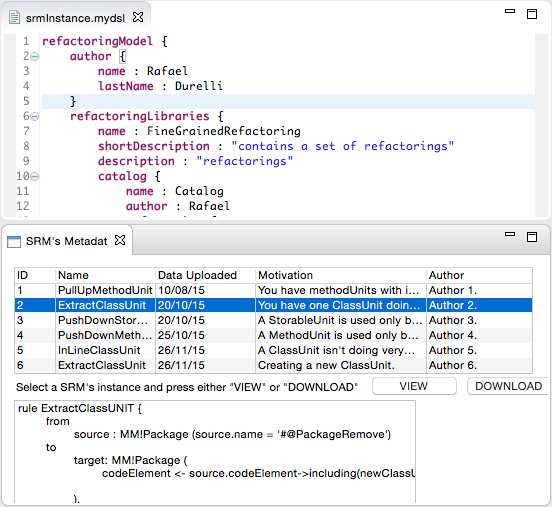
\includegraphics[scale=0.6]{images/DOWNLOAD_KDM_RE}
	\fautor
\end{figure}


\section{Módulo de Sincronização}\label{sec:modulo_de_sincronizacao_kdm_re}

Usualmente, durante o desenvolvimento e modernização de software seguindo as diretrizes e passos da abordagem MDE, o software geralmente é modelado e representado utilizando diferentes instâncias de metamodelos para representar as visões e todos os artefatos de um sistema. Em outras palavras, geralmente existem metamodelos para abstrair e representar todos os artefatos do sistema, tais como: metamodelos para o código-fonte, metamodelos para representar e abstrair o banco de dados, metamodelos para representar e abstrair a arquitetura do sistema, etc. Como apresentado no Capítulo~\ref{chapter:fundamentacao_teorica} o metamodelo KDM é capaz de agrupar todos esses artefatos em um único metamodelo, sendo assim, possível de representar diferentes visões/artefatos e seus relacionamentos de um determinado sistema em uma única instância do metamodelo KDM. Porém, conforme o engenheiro de software aplica um conjunto de refatorações em uma determinada instância do metamodelo KDM mudanças são realizadas. Usualmente tais mudanças podem necessitar que subsequentes alterações sejam realizadas para que outras visões/artefatos do metamodelo KDM fiquem consistentes e sincronizados.

Neste contexto, uma premissa fundamental é manter todas as visões/artefatos do metamodelo KDM sincronizados durante todo o processo de modernização do software. Dessa forma, quando as visões/artefatos representados em nível de modelos são alterados, é de extrema importância realizar um conjunto de propagação de mudança por todas as visões/artefatos para mantê-los atualizados e sincronizados, espelhando assim, a alteração em todas as visões/artefatos do software. Usualmente, como apresentado nos Capítulo~\ref{chapter:fundamentacao_teorica}, Seção~\ref{sec:refatoracao} e Capítulo~\ref{chapter:catalogo_refactoring_KDM} essas alterações podem ser realizadas por meio de refatorações, as quais são atividades centrais durante o processo de modernização. Porém, quando um software é representado utilizando diferentes abstrações e visões em nível de modelos, um acidente comum que pode ocorrer durante a atividade de refatoração é a dessincronização dessas visões, fazendo com que as visões/artefatos que representam o sistema fiquem inconsistente após a atividade de refatoração. Uma forma de resolver esse problema é aplicar técnicas de propagação de mudança, cujo objetivo é identificar e atualizar todas as instâncias dependentes dos elementos que foram refatorados. % No entanto, a maioria das propostas de propagação de mudança foram desenvolvidas para propagarem mudanças em diferentes metamodelos, além disso, usualmente tais metamodelos são de diferentes fornecedores dificultando o entendimento e a programação de mudança (ref). 
Diante deste contexto, a ferramenta KDM-RE possui um módulo de sincronização para realizar a propagação de mudança e preservação de comportamento após a aplicação de refatorações em instâncias do metamodelo KDM. Utilizando esse módulo, engenheiros de software podem se concentrar apenas na aplicação das refatorações ou reutiliza-las por meio do metamodelo SRM (ver Capítulo~\ref{chapter:Toward_a_Refactoring_Metamodel_for_KDM}), sem terem que se preocuparem com a propagação de mudanças para outras visões/artefatos do metamodelo KDM. 

É importante destacar que o fluxo desse módulo de sincronização inicia-se considerando que o engenheiro de software almeja aplicar um conjunto de refatorações em um sistema que está já representado por meio de uma instância do metamodelo KDM. Essa instância do metamodelo KDM deve ser a mais completa possível, ou seja, represente todas as visões/artefatos do sistema, desde o código-fonte até os elementos arquiteturais do sistema\footnote{Na verdade é importante que mais de uma visão/artefato seja representado utilizando o metamodelo KDM, seja código-fonte, banco de dados, elementos estruturais, etc.}. Após o engenheiro de software aplicar uma determinada refatoração, o módulo de sincronização, a qual contém três principais passos, efetivamente é iniciado. De forma resumida pode-se descrever os três passos do módulo da seguinte forma. 

O primeiro passo realiza uma comparação (do inglês - \textit{diff}) entre a instância refatorada do metamodelo KDM com a instância do metamodelo KDM original, ou seja, a instância do metamodelo KDM antes do engenheiro de software aplicar a refatoração. Como resultado, esse passo cria uma lista que contém todas as instâncias das metaclasses do KDM que sofreram uma modificação durante a refatoração quando comparado com a instância do KDM original. Em seguida, o segundo passo utiliza como entrada a lista gerada para ser utilizada como parâmetro para um algoritmo de mineração e identificação de dependências. Esse algoritmo tem como objetivo identificar todas as instâncias das metaclasses do KDM que possuem dependência com as metaclasses refatoradas. Como resultado, esse algoritmo também cria uma lista, a qual é utilizada no terceiro passo. O terceiro passo utiliza a lista criada pelo algoritmo para realizar um conjunto de transformações em nível de modelo. Tais transformações foram pré-definidas e representam as propagações de mudanças por todas as visões do KDM. É importante destacar que o módulo de sincronização da KDM-RE foi implementada com a preocupação de ser uma forma genérica e desacoplada. Assim, esse módulo pode ser aplicado em um grande conjunto de refatorações fazendo com que o engenheiro de software não tenha que se preocupar com a propagação de mudança para outras visões/artefatos do KDM. 

%Para exemplificar os três principais passos do módulo de sincronização essa
%As demais seções deste capítulo estão organizadas da seguinte forma: na Seção~\ref{sec:kdm_sinc} a abordagem KDM-SInc é descrita, na Subseção~\ref{sec:diff_entre_kdm} o primeiro passo da abordagem KDM-SInc é apresentado, o segundo passo é apresentado na SubSeção~\ref{subsec:identificandoPontoParaExecutarApropagacao}, e na Subseção~\ref{subsec:aplicar_propagacao_KDM-SInc}. Na Seção~\ref{sec:consideracoes_finals_kdm_sinc} as considerações finais deste capítulo são apresentadas.


%\section{A Abordagem KDM-SInc}\label{sec:kdm_sinc}

Como já mencionado, um problema critico durante a modernização de software diz respeito a propagação de mudança - por exemplo, dado um conjunto de refatorações que são aplicadas durante a modernização de software é importante identificar quais são as mudanças que precisam ser realizadas para manter a consistência e sincronia de todos os artefatos do sistema. Dessa forma, propagação de mudança é uma técnica de extrema importância durante a elaboração de processo de modernização de software. O engenheiro de software tem que ter a certeza que a refatoração foi corretamente propagada e que o software não possui nenhuma inconsistência. Embora muitas abordagens de propagações de mudanças possam ser identificadas na literatura, a propagação de mudanças ainda é um desafio durante a manutenção e modernização de software~\cite{Tom_2008_roadmap}. Além disso, a maioria das abordagens de propagação de mudanças existentes têm como principal artefato o código-fonte~\cite{Vaclav_methodology, Deursen07model_drivensoftware}. Similarmente também é possível identificar algumas abordagens que dão suporte para a propagação de mudança para o metamodelo UML~\cite{Egyed_2008,Liu02rule, Briand_2006}. Porém, até o momento nenhuma iniciativa foi criada para o metamodelo KDM. Para suprir essa limitação nessa a KDM-RE possui um módulo de sincronização. Esse módulo de sincronização tem como objetivo propagar mudanças por todas as visões/artefatos do metamodelo KDM para mantê-lo atualizado e sincronizado após a aplicação de uma refatoração. A intenção é criar um apoio computacional que mantenha uma determinada instância do metamodelo KDM consistente e sincronizada entre todas as visões/artefatos do metamodelo KDM após a aplicação de uma determinada refatoração. 

\begin{figure}[h]
	\centering
	% Requires \usepackage{graphicx}
	\caption{Visão Geral da Abordagem KDM-SInc.}
	\label{fig:kdm_sinc}
	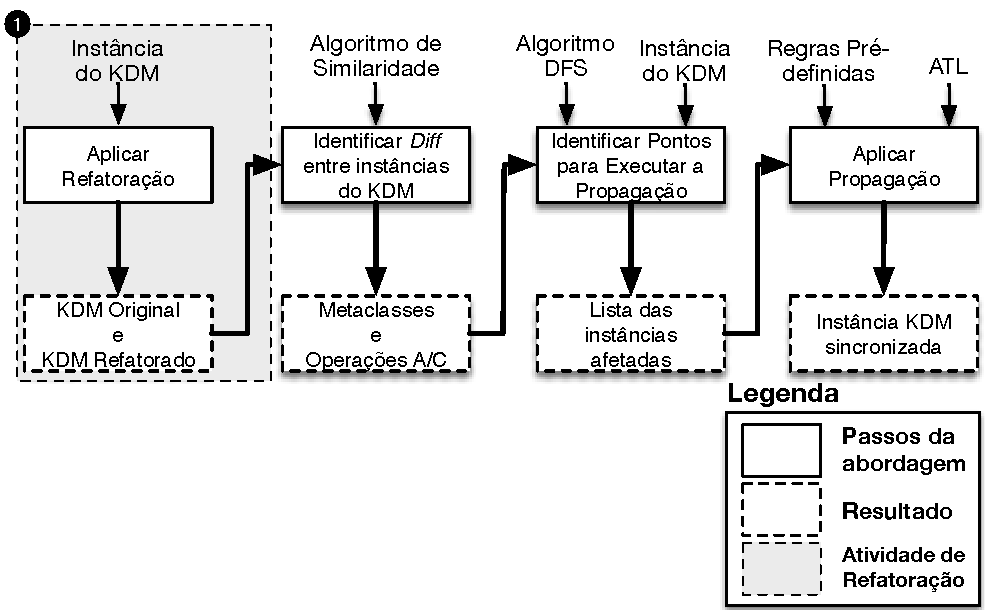
\includegraphics[scale=0.65]{images/AbordagemKDM_SInc}
	\fautor
\end{figure}


Na Figura~\ref{fig:kdm_sinc} é apresentado uma visão geral do módulo de sincronização. Como pode ser observado o módulo de sincronização contempla três principais passos. Antes dos passos do módulo se iniciarem uma atividade de refatoração deve ser realizada. Essa atividade esta representada na caixa cinza da Figura~\ref{fig:kdm_sinc} \ding{202} e é apoia pelo módulo de refatoração apresentado na Seção~\ref{sec:modulo_de_refatoracao_kdm_re}. A atividade de refatoração esta fora do escopo do módulo de sincronização, assim, é de responsabilidade do engenheiro de software aplicar e/ou reutilizar refatoração para o metamodelo KDM e executa-lá em uma instância do metamodelo KDM. A única restrição do módulo de sincronização da KDM-RE é que duas versões da instância do metamodelo KDM seja utilizada como entrada - uma versão que representa a instância do metamodelo KDM antes da aplicação das refatorações (\aspas{instância original}) e outra versão que representa uma instância do metamodelo KDM após a aplicação de \textit{n} refatorações (\aspas{instância refatorada}). Note que uma \aspas{instância original} do metamodelo KDM, é aquela que ainda não foi refatorada, também denominada de \aspas{KDM esquerdo}, similarmente, a \aspas{instância refatorado} do metamodelo KDM pode ser entendida como \aspas{KDM direito}. 

Após a aplicação de um conjunto de refatorações o primeiro passo do módulo de sincronização é iniciado. Nesse passo uma comparação (\textit{diff}) entre a instância original e a instância refatorada é realizada. Como resultado desse passo uma lista é crida. Essa lista contém todas as instâncias das metaclasses do KDM que sofreram alguma modificação durante a refatoração quando comparado com a instância do KDM original. Além disso, essa lista também especifica qual(is) foi(ram) a(s) modificação(ões) realizada(s). Por exemplo, se na versão refatorada (\aspas{KDM direito}) uma nova instância da metaclasse \texttt{ClassUnit} foi adicionada a lista irá conter duas importantes informações: (\textit{i}) a instância da metaclasse \texttt{ClassUnit} e (\textit{ii}) qual operação foi realizada, nesse exemplo \texttt{add} \texttt{ClassUnit}. Essas duas informações são importantes para identificar o que foi alterado e qual operação foi realizada (neste caso uma \texttt{ClassUnit} foi adicionada) - assim, é possível identificar quais propagações devem ser realizadas nas outras visões/pacotes do metamodelo KDM.

Em seguida, o segundo passo do módulo de sincronização é iniciado. Esse passo identifica todas as metaclasses que precisam ser sincronizadas/atualizadas após a aplicação da refatoração. Esse passo utiliza o algoritmo de busca em profundidade (do inglês - \sigla{DFS}{\textit{Depth-First Search}}). O algoritmo DFS foi alterado para utilizar os seguintes parâmetros como entrada: (\textit{i}) a lista criada no primeiro passo e (\textit{ii}) a instância refatorado do KDM (\aspas{KDM direito}). Utilizando a instância refatorado o algoritmo DFS identifica e cria uma lista que contém todas as metaclasses que possuem dependência com as metaclasses que efetivamente foram refatoradas.

Posteriormente o utlimo passo pode ser iniciado para realizar a propagação de mudanças na instância do KDM. Como entrada esse passo utiliza todas as metaclasses que possuem dependência com as metaclasses que foram refatoradas (lista criada no passo anterior). As propagações de mudanças são um conjunto de regras pré-definidas que são realizadas de acordo com a instância alterada (\texttt{Package}, \texttt{ClassUnit}, \texttt{MethodUnit}, \texttt{StorableUnit}, etc) e sua operação atômica (\texttt{add}, \texttt{delete} e \texttt{change}). Após o término desse último passo todas as visões/artefatos da instância do KDM estão sincronizadas e consistentes.

%É importante salientar que os três passos do módulo de sincronização são executados várias vezes até que não haja mais elementos que precisem ser atualizados/sincronizados. Esse ciclo é necessário uma vez que uma determinada instância do metamodelo KDM pode ainda exigir propagações em outros artefatos/visões, por isso, cada ciclo da abordagem KDM-SInc se concentra apenas no próximo nível de propagação. A condição de parada da abordagem KDM-SInc é quando o algoritmo DFS, definido no segundo, retornar uma lista vazia, indicando que não há mais elementos que precisam ser modificados.

Para auxiliar a elaboração do primeiro passo do módulo de sincronização o \textit{framework} EMFCompare\footnote{https://www.eclipse.org/emf/compare/} foi estendido para comparar instâncias do metamodelo KDM. O segundo passo é apoiado por um motor de busca cuja parte central é o algoritmo DFS juntamente com um conjunto de expressões definidas em linguagem de buscas que são executadas em uma instância do metamodelo KDM para obter todos os pacotes do KDM. O último passo do módulo de sincronização é apoiado por um motor de propagação, o qual utiliza um conjunto de regras pré-definidas e implementadas em ATL para executar as propagações. Todas as propagações foram definidas com base nas instâncias das metaclasses alteradas juntamente com as operações atômicas (\texttt{add}, \texttt{delete} e \texttt{change}) apresentadas no Capítulo~\ref{chapter:catalogo_refactoring_KDM}. Maiores detalhes sobre da passo do módulo de sincronização são apresentados a seguir. %Porém, detalhes técnicas da abordagem KDM-SInc são omitidos nesse capítulo. Informações técnicas sobre a abordagem KDM-SInc são salientadas no Capítulo X onde o apoio computacional KDM-RE é apresentado, mais especificadamente na Seção X, onde o módulo de propagação é apresentado.

%Para auxiliar a elaboração do passo [A] o \textit{framework} EMFCompare\footnote{https://www.eclipse.org/emf/compare/} foi estendido para comparar instâncias do metamodelo KDM. O passo [B] é tecnicamente apoiado por um motor de busca cuja parte central é o algoritmo DFS juntamente com um conjunto de expressões definidas em XPath que são executadas em uma instância do metamodelo KDM para obter todos os pacotes do KDM. Finalmente, o passo [C] é apoiado por um motor de propagação, o qual utiliza um conjunto de transformações pré-definidas em ATL para executar as propagações. Todas as propagações foram definidas com base nas operações atômicas (\texttt{add}, \texttt{delete} e \texttt{change}) apresentadas no Capítulo X \change{Mudar aqui}. Dessa forma, quando um conjunto de refatorações são executadas um conjunto de propagações bem definidas podem ser executadas no contexto de instâncias do metamodelo KDM. Maiores detalhes sobre da passo da abordagem KDM-SInc são apresentados nas próximas seções.

\subsection{Identificar \textit{Diff} entre Instâncias do Metamodelo KDM}\label{sec:diff_entre_kdm}

Nessa seção o primeiro passo do módulo de sincronização é apresentado e discutido. Como já salientado o primeiro passo é apoiado pelo \textit{framework} EMFCompare. Esse \textit{framework} foi escolhido pois o mesmo pode ser facilmente adaptado, estendido e implementa um algoritmo de similaridade de instâncias de metamodelo eficiente. A fim de entender melhor como o primeiro passo do módulo de sincronização funciona, considere os seguintes três sub-passos: (\textit{i}) \textit{Matching}, (\textit{ii}) \textit{Diffing} e (\textit{iii}) Análise dos \textit{Diffs} como apresentado na Figura~\ref{fig:diff_emf_compare}. 

\begin{figure}[h]
	\centering
	% Requires \usepackage{graphicx}
	\caption{Visão Geral da Execução do Primeiro Passo da Abordagem KDM-SInc.}
	\label{fig:diff_emf_compare}
	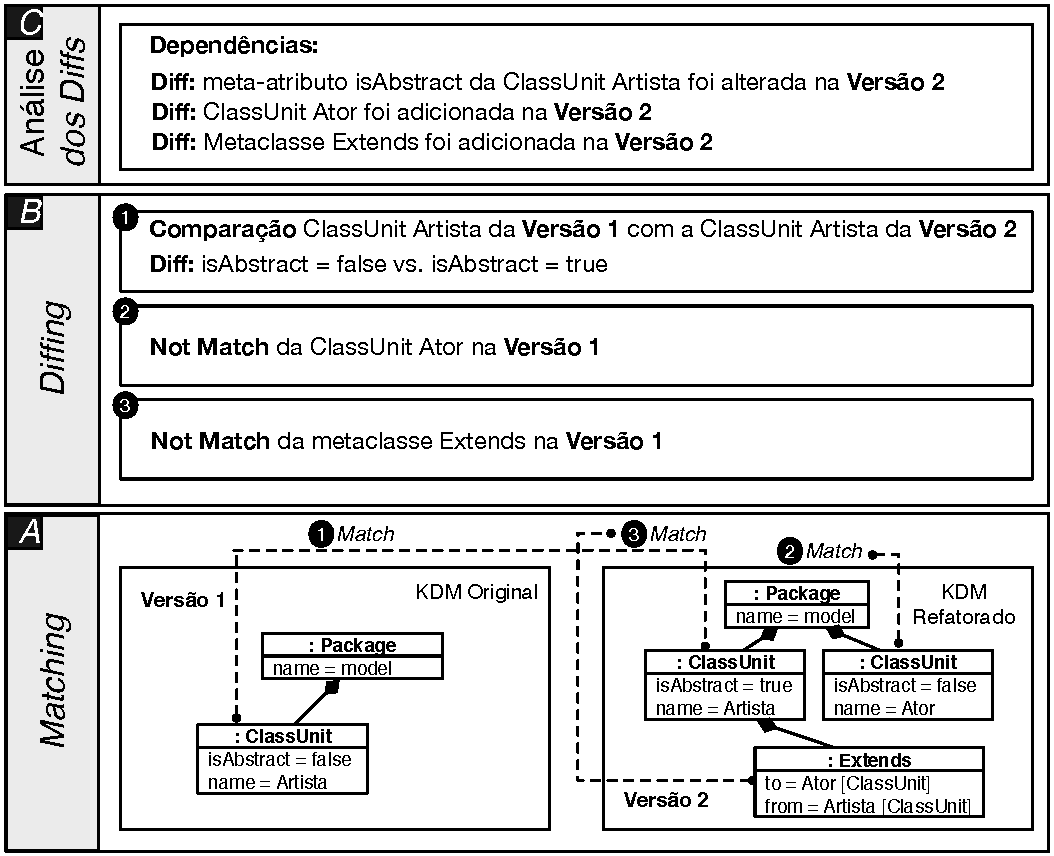
\includegraphics[scale=0.7]{images/matching_diffing_analise_3}
	\fautor
\end{figure}

Com pode ser observado na Figura~\ref{fig:diff_emf_compare} o primeiro sub-passo, \textit{matching}, necessita de duas instâncias do metamodelo KDM - uma instância original (\aspas{KDM esquerdo}), denominada \textbf{versão 1} na Figura~\ref{fig:diff_emf_compare}, e uma instância refatorada (\aspas{KDM direito}), \textbf{versão 2} na Figura~\ref{fig:diff_emf_compare}. Dado essas duas instâncias do KDM, os correspondentes elementos nas duas versões do metamodelo KDM são identificados. Em uma instância do KDM cada elemento possui um identificar único, não volátil e persistente. Portanto, os correspondentes elementos são identificados por meio desses identificadores únicos tais como XMI IDs. Por exemplo, ainda analisando a Figura~\ref{fig:diff_emf_compare} pode-se observar que a instância da metaclasse \texttt{ClassUnit} \aspas{Artista} apresentada na \textbf{versão 1} corresponde a instância da metaclasse \texttt{ClassUnit} \aspas{Artista} na \textbf{versão 2}. Para as instâncias das metaclasses \texttt{ClassUnit} \aspas{Ator} e \texttt{Extends} na \textbf{versão 2}, no entanto, nenhum elemento correspondente foi identificado na \textbf{versão 1}. Note que para cada elemento correspondente identificado, ou não identificado, um elemento \textit{match} é criado e será utilizado no sub-passo seguinte.

No segundo sub-passo, \textit{Diffing}, todos os correspondentes elementos identificados são examinados para identificar diferenças em seus meta-atributos. Para cada diferença identificada um objeto \textit{diff} é criado, o qual descreve com precisão cada diferença identificada entre os correspondentes elementos. Por exemplo, ainda considerando a Figura~\ref{fig:diff_emf_compare}, quando a instância da metaclasse \texttt{ClassUnit} \aspas{Artista} da \textbf{versão 1} e \textbf{versão 2} são examinadas é possível observar que o meta-atributo \texttt{isAbstract} possui o valor \textit{false} na \textbf{versão 1}, enquanto que na \textbf{versão 2} o mesmo meta-atributo o valor é \textit{true} - representa a operação \texttt{change}. Instâncias de metaclasses que não contêm elementos correspondentes em ambas as versões são consideradas adicionadas ou deletadas (\texttt{add} e \texttt{delete}) - a operação é identificada dependendo da direção, por exemplo, se uma instância de uma metaclasse apenas existe do lado direito (\aspas{KDM direito}) essa instância foi adicionada, por outro lado, se uma instância apenas existe do lado esquerdo (KDM esquerdo) essa instância foi deletada. Na Figura~\ref{fig:diff_emf_compare} é possível identificar que duas instâncias foram adicionadas - uma instância da metaclasse \texttt{ClassUnit} denominada Ator e uma instancia da metaclasse \texttt{Extends}.

%Detecting refactorings may be realized by tracking the user’s operations. Operation-based conflict detection is very precise, because every change is recorded and the complete operation sequence may be replayed in the correct order.


Em seguida o terceiro sub-passo, Análise dos \textit{Diffs} é executado. Nesse sub-passo todos os objetos \textit{diffs} criados anteriormente são examinados para criar uma lista de dependência contendo as instâncias das metaclasses alteradas e quais operações foram realizadas. No exemplo apresentado na Figura~\ref{fig:diff_emf_compare} a lista criada possui três dependências. A primeiro dependência informa que o meta-atributo \texttt{isAbstract} da metaclasse \texttt{ClassUnit} Artista da \textbf{versão 1} foi alterado (\texttt{change}) de \textit{false} para \textit{true} na \textbf{versão 2}. A segunda dependência ilustra que uma instância da metaclasse \texttt{ClassUnit} Ator foi adicionada (\texttt{add}) na \textbf{versão 2} e a terceira dependência representa que uma instância da metaclasse \texttt{Extends} foi adicionada na \textbf{versão 2}.


\subsection{Identificar Pontos para Executar a Propagação}\label{subsec:identificandoPontoParaExecutarApropagacao}

Nessa seção o segundo passo do módulo de sincronização é apresentado. Esse passo resume-se basicamente na adaptação do algoritmo DFS para identificar todas as metaclasses que precisam ser sincronizadas/atualizadas após a aplicação da refatoração. Esse algoritmo utiliza como entrada a lista criada no passo anterior. Como as instâncias do metamodelo KDM são persistidas utilizando a padronização XMI o algoritmo precisa de uma forma para buscar as dependências nesse XMI. Assim, esse passo utiliza expressões em XPath~\cite{kay2011xslt} que são executadas na instância do metamodelo KDM para obter todos os pacotes do KDM. Por exemplo, na Figura~\ref{fig:xpath_queries} é apresentado algumas expressões definidas em XPath que são utilizadas antes da aplicação do algoritmo DFS. A primeira expressão retorna a metaclasse \texttt{Segment} que é o elemento inicial de qualquer instância do metamodelo KDM. As outras expressões ilustradas nas linhas 2-5 representam os outros pacotes do metamodelo KDM. Os elementos retornados nas expressões XPath são também utilizadas como entrada para o algoritmo DFS.

\begin{figure}[h]
	\centering
	% Requires \usepackage{graphicx}
	\caption{Expressões definidas em XPath para obter os pacotes do KDM.}
	\label{fig:xpath_queries}
	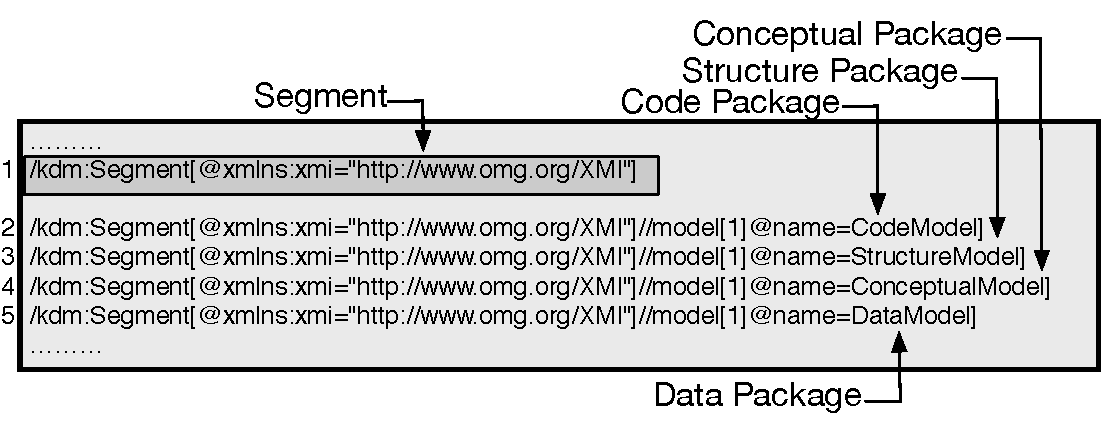
\includegraphics[scale=0.68]{images/queiresANDATLSBESNew}
	\fautor
\end{figure}

O Algoritmo~\ref{alg:death1} ilustra como o DFS identifica todas as metaclasses que precisam ser sincronizadas/atualizadas após a aplicação da refatoração. A Figura~\ref{fig:dfsalg} apresenta como é o funcionamento do algoritmo DFS. Cada nó representa uma instância de uma metaclasse do metamodelo KDM e os vértices representam os relacionamentos entre as instâncias das metaclasses, por exemplo, o nó \texttt{A} representa uma instância da metaclasse \texttt{Segment} e os nós \texttt{K}, \texttt{H}, \texttt{E} e \texttt{B} representam instâncias das metaclasses \texttt{CodeModel}, \texttt{StructureModel}, \texttt{ConceptualModel} e \texttt{DataModel}, respectivamente. Mais especificadamente, o algoritmo funciona da seguinte forma: primeiro é necessário escolher um ponto inicial de partida, no caso do módulo de sincronização o ponto inicial é a instância da metaclasse \texttt{Segment}, metaclasse raiz de qualquer instância do metamodelo KDM. Em seguida, a instância da metaclasse \texttt{Segment} deve ser visitada, adicionada em uma pilha e marcada como visitada. Posteriormente, o algoritmo visita uma outra instância de outra metaclasse que ainda não foi visitada e verifica se a mesma possui uma associação do tipo \texttt{implementation}. Caso afirmativo, o algoritmo deve verificar se essa associação possui referência para algum elemento identificado na lista gerada no primeiro passo, caso a associação contenha um elemento o mesmo deve ser adicionado em outra pilha e marcado como visitado. Todo esse processo continua até que o algoritmo alcance a última metaclasse instanciada no KDM. 

\begin{algoritmo}[h]
     \SetAlgoLined
     \KwIn{DFS (G, u) onde \textit{G} é uma instância do  KDM, \textit{u} é a metaclasse inicial obtida pela expressão XPath, ou seja, \texttt{Segment}}
     \KwOut{Uma coleção de metaclasses que precisam ser sincronizadas}
     \Begin{
     \ForEach{$outgoing$ edge e = (u, v) of u} {
	\If{vertex v as has not been visited}{
			\If{vertex v contain implementation = true }{
				
				\ForEach{$implementations$ element}{
				verify all elements in implementation
				}
				Mark vertex v as visited (via edge e).
				Recursively call DFS (G, v).
			}
			
				}				
			}		
	
	}
     \caption{Algoritmo DFS.}
     \label{alg:death1}
   \end{algoritmo}

\begin{figure}[h]
	\centering
	% Requires \usepackage{graphicx}
	\caption{Funcionamento do Algoritmo DFS.}
	\label{fig:dfsalg}
	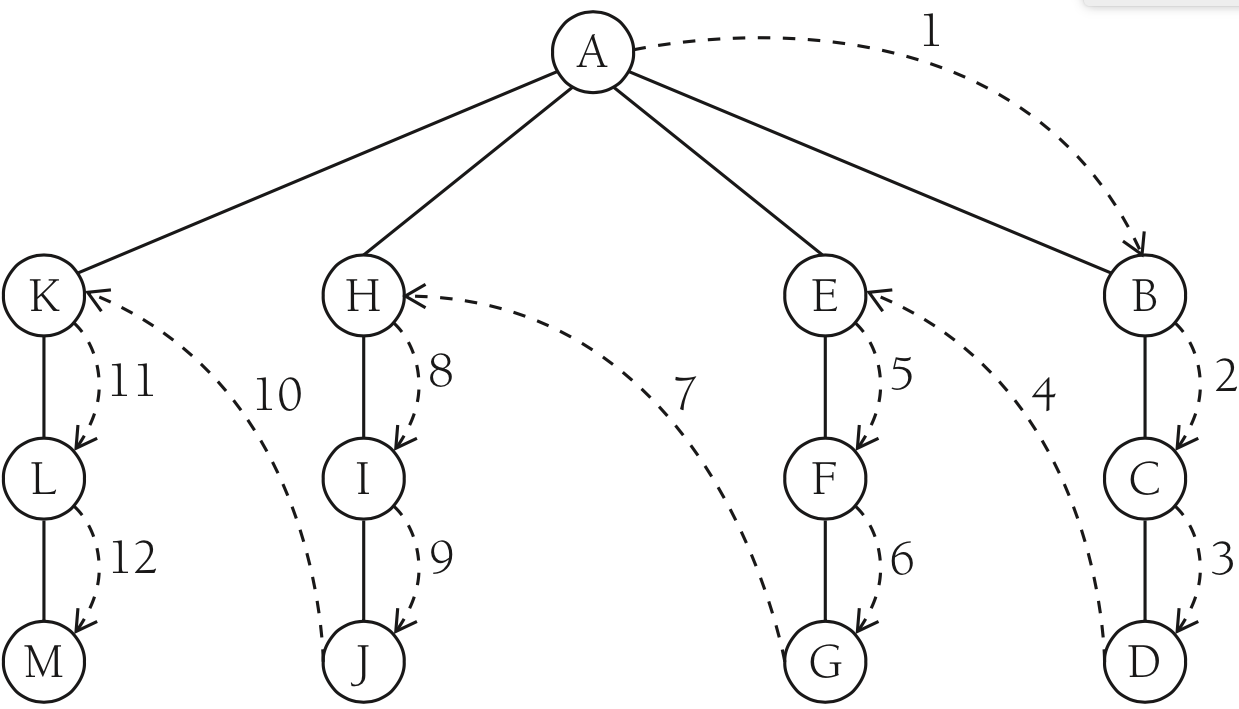
\includegraphics[scale=0.3]{images/algWorks2}
	\fautor
\end{figure}

Em seguida o algoritmo ainda verifica se a instância da metaclasse \texttt{Segment} possui alguma instância adjacente que ainda não foi marcada como visitado. Caso o algoritmo identifique uma instância de metaclasse adjacente ainda não visitada todo o processo é iniciado novamente, sempre verificando a associação \texttt{implementation}. Quando o algoritmo finalmente alcança a última instância da metaclasse, ou seja, todas as instâncias de metaclasse do KDM foram visitadas e verificadas corretamente, o algoritmo cria uma lista contendo todas as instâncias das metaclasses afetadas na refatoração. 

\subsection{Aplicar Propagação}\label{subsec:aplicar_propagacao_KDM-SInc}
Nesta seção o terceiro passo do módulo de sincronização é apresentado. Esse passo objetiva realizar as mudanças e propagações necessárias para manter uma determinada instância do metamodelo KDM sincronizada e consistente. A sincronização é importante para o metamodelo KDM uma vez que o mesmo possui metaclasses que contêm conexões diretas com outras metaclasses de outras visões/artefatos do KDM. Assim, manter a instância do metamodelo KDM sincronizado e consistente após a aplicação de uma refatoração é importante. 

No contexto desta Tese, como apresentado no Capítulo~\ref{chapter:catalogo_refactoring_KDM}, as refatorações que são criadas para o metamodelo KDM são refatorações de baixa granularidade e que são aplicadas diretamente na camada \texttt{Code} do metamodelo KDM. Porém, uma determinada refatoração pode demandar outras modificações que deveriam ser realizadas em outros camadas/visões do metamodelo KDM para mantê-lo consistente e sincronizado. Por exemplo, considere a refatoração \textit{Rename Package} - o nome de um determinado pacote é alterado de PacoteX para PacoteY, se uma instância da metaclasse \texttt{Layer}\footnote{Metaclasse definida no pacote \texttt{Structure} do metamodelo KDM para representar camadas em nível arquitetural.} é utilizada para representar o pacote em nível arquitetural, então essa mesma instância da metaclasse \texttt{Layer} também deve-se ser renomeada. 

Esse passo utiliza um conjunto de regras pré-definidas que são iniciadas de acordo a(s) refatoração(ões) aplicada(s) na instância do metamodelo KDM. Mais especificadamente, todas as propagações especificadas nesse passo são pré-definidas para serem disparadas após a aplicação de específicas refatorações. Todas as propagações são definidas com base nas mudanças realizadas em uma determinada instância de metaclasses do metamodelo KDM. Além disso, todas as regras pré-definidas foram implementadas em ATL. No Apêndic~\ref{apendice:regras_propagacao} nas Tabelas~\ref{tab:propagacaoes_kdm_sinc_package},~\ref{tab:propagacaoes_kdm_sinc_classUnit},~\ref{tab:propagacaoes_kdm_sinc_StorableUnit} e \ref{tab:propagacaoes_kdm_sinc_method} todas as regras de programação pré-definidas são explicadas.  

\subsection{Exemplo de execução do Módulo de Sincronização}

Como apresentado no Capítulo~\ref{chapter:catalogo_refactoring_KDM} a refatoração \texttt{Extract ClassUnit} pode ser criada por um conjunto de duas operações atômicas: \texttt{add} e  \texttt{delete}. Dessa forma, o módulo de sincronização identifica que a refatoração \texttt{Extract ClassUnit} executou um conjunto de operações atômica (\texttt{add} e \texttt{delete}) e cria uma lista para ser utilizada no passo seguinte. No contexto da refatoração \texttt{Extract ClassUnit} apresentada na Figura~\ref{fig:kdm_re_wizard_extract_class} as seguintes operações foram realizadas: 

\begin{itemize}

\item \texttt{add} uma instância de \texttt{ClassUnit} denominada \texttt{Document};

\item \texttt{delete} uma instância de \texttt{StorableUnit} denominada CPF da \texttt{ClassUnit} \texttt{Cliente};

\item \texttt{add} uma instância de \texttt{StorableUnit} na \texttt{ClassUnit} \texttt{Document};

\item \texttt{add} uma instância de \texttt{StorableUnit} do tipo \texttt{Document} na \texttt{ClassUnit} \texttt{Cliente};

\item \texttt{add} duas instância de \texttt{MethodUnit} para representar os métodos assessores na \texttt{ClassUnit} \texttt{Cliente}.
\end{itemize}

Em seguida o módulo de sincronização executa o algoritmo DFS para identificar todas as metaclasses que precisam ser sincronizadas/atualizadas após a aplicação da refatoração. Esse algoritmo utiliza como entrada a lista criada no passo anterior. Expressões definidas em XPath são utilizadas para navegar em todas as visões da instância do metamodelo KDM. Ao término da execução desse algoritmo, o mesmo irá criar uma lista que contém todas as instâncias das metaclasses afetadas na refatoração. 
   

O terceiro passo do módulo de sincronização objetiva realizar as mudanças e propagações necessários para manter uma determinada instância do metamodelo KDM sincronizada e consistente. Utilizando a lista de operações realizadas na refatoração e a lista que possui os elementos afetados na refatoração o módulo de programação utiliza um conjunto de regras pré-definidas para realizar a propagação. Todas as propagações estão apresentadas nas Tabelas~\ref{tab:propagacaoes_kdm_sinc_package},~\ref{tab:propagacaoes_kdm_sinc_classUnit},~\ref{tab:propagacaoes_kdm_sinc_StorableUnit} e~\ref{tab:propagacaoes_kdm_sinc_method} do Apêndice~\ref{apendice:regras_propagacao}. Para a refatoração \texttt{Extract ClassUnit} utilizada como exemplo as propagações que serão realizadas são:

\begin{figure}[!h]
	\centering
	% Requires \usepackage{graphicx}
	\caption{Instância antes e após a abordagem KDM-SInc.}
	\label{fig:efeitoPropagacaoKDMSINC}
	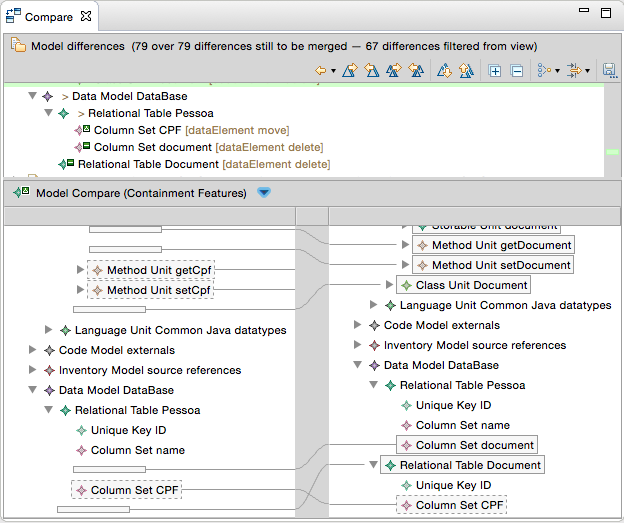
\includegraphics[scale=0.6]{images/propagacaoKDMEfeito}
	\fautor
\end{figure}

\begin{itemize}
    \item \texttt{add} uma instância de \texttt{RelationalTable} com o meta-atributo \texttt{name} denominada \texttt{Document};
    
    \begin{itemize}
        \item \texttt{add} uma instância da metaclasse \texttt{UniqueKey} na instância \texttt{RelationalTable} criada;
    \end{itemize}
    
    \item \texttt{delete} uma instância de \texttt{ColumnSet} denominada CPF da \texttt{RelationalTable} \texttt{Pessoa};
    
    \item \texttt{add} uma instância de \texttt{ColumnSet} com o meta-atributo \texttt{name} denominado CPF na instância da metaclasse \texttt{RelationalTable} \texttt{Document};
    
    \item \texttt{add} uma instância de \texttt{ColumnSet} do com o meta-atributo \texttt{name} denominado \texttt{document} na \texttt{RelationalTable} \texttt{Pessoa};

    %\item \texttt{add} duas instância de \texttt{MethodUnit} para representar os métodos assessores na \texttt{ClassUnit} \texttt{Cliente}.
    
\end{itemize}

Adicionalmente, a KDM-RE fornece uma forma de visualizar graficamente se as propagações foram realmente executadas. Por exemplo, considere a Figura~\ref{fig:efeitoPropagacaoKDMSINC}. Essa figura representa duas instâncias do metamodelo KDM. A instância apresentada do lado esquerdo é denominada \textbf{versão 1} e equivale a instância antes (original) de aplicar o módulo de sincronização. A instância do lado direito é intitulada de \textbf{versão 2} e representa uma instância do metamodelo KDM sincronizada e propagada de acordo os passos e regras definidas pela abordagem KDM-SInc.% nas Tabelas~\ref{tab:propagacaoes_kdm_sinc_package},~\ref{tab:propagacaoes_kdm_sinc_classUnit},~\ref{tab:propagacaoes_kdm_sinc_StorableUnit} e~\ref{tab:propagacaoes_kdm_sinc_method}.





%Como observado a instância apresentada do lado direito da Figura~\ref{fig:efeitoPropagacaoKDMSINC} representa a instância do metamodelo KDM sincronizada e propagada. 


%A sincronização é importante para o metamodelo KDM uma vez que o mesmo possui metaclasses que contêm conexões diretas com outras metaclasses de outras visões/artefatos do KDM. Assim, manter a instância do metamodelo KDM sincronizado e consistente após a aplicação de uma refatoração é importante. 

%No contexto desta Tese, como apresentado no Capítulo~\ref{chapter:catalogo_refactoring_KDM} as refatorações que são definidas e adaptadas para o metamodelo KDM são refatorações de baixa granularidade e que são aplicadas diretamente na camada \texttt{Code} do metamodelo KDM. Porém, uma determinada refatoração pode demandar outras modificações que deveriam ser realizadas em outros camadas/visões do metamodelo KDM para mantê-lo consistente e sincronizado. Por exemplo, considere a refatoração \textit{Rename Package} - o nome de um determinado pacote é alterado de PacoteX para PacoteY, se uma instância da metaclasse \texttt{Layer}\footnote{Metaclasse definida no pacote \texttt{Structure} do metamodelo KDM para representar camadas em nível arquitetural.} é utilizada para representar o pacote em nível arquitetural, então essa mesma instância da metaclasse \texttt{Layer} também deve-se ser renomeada. 

%Diferentemente da atividade de refatoração apresentada no Capítulo~\ref{chapter:catalogo_refactoring_KDM} onde o engenheiro de modernização precisa escolher qual refatoração aplicar na instância do metamodelo KDM ou reutilizar um refatoração utilizando o metamodelo SRM apresentado no Capítulo~\ref{chapter:Toward_a_Refactoring_Metamodel_for_KDM}, esse passo utiliza um conjunto de regras pré-definidas que são iniciadas de acordo a(s) refatoração(ões) aplicada(s) na instância do metamodelo KDM. Mais especificadamente, todas as propagações especificadas nesse passo são pré-definidas para serem disparadas após a aplicação de específicas refatorações. Algumas propagações são realizadas sem a interferência do engenheiro de modernização, no entanto, existem propagações que precisam de informações importantes para realizar consistentemente a propagação. Assim, algumas propagações podem ser realizadas de forma totalmente automática, enquanto outras precisam de algumas informações antes de executar a propagação propriamente dita.

%Esse passo da abordagem KDM-SInc utiliza um conjunto de regras pré-definidas para propagar todas as mudanças em uma instância do metamodelo KDM com o intuito de mantê-lo consistente e sincronizado com todas as visões/artefatos. Todas as propagações são definidas com base nas mudanças realizadas em um determinada instância de metaclasses do metamodelo KDM. A abordagem KDM-SInc 

%Por exemplo, considere a Figura~\ref{fig:extractClassRefactoring} onde o engenheiro de modernização está aplicando a refatoração \texttt{Extract ClassUnit} em uma instância de \texttt{ClassUnit} denominada \texttt{Pessoa}. O primeiro passo do módulo de sincronização irá realiazar uma comparação entre a instância refatorada e a instância original do metamodelo KDM. Como apresentado no Capítulo X\change{mudar} a refatoração \texttt{Extract ClassUnit} é uma refatoração composta, assim, é necessário aplicar um conjunto de operações atômicas: \texttt{add}, \texttt{delete} e \texttt{change}.

\section{Trabalhos Relacionados}

Nesta seção, são descritos os principais trabalhos relacionados com ferramentas que aplicam refatorações em nível de modelos encontradas na literatura. Foram identificadas algumas ferramentas que nortearam o desenvolvimento da KDM-RE, assim, nesta seção, são mostradas as principais semelhanças e diferenças encontradas.

\citeonline{arendt2013tool} em seu artigo propõem uma ferramenta denominada EMF Refactor para aplicar refatorações em modelos EMF. Na Figura~\ref{fig:arquitetura_emf_refactor}, é apresentada a arquitetura da ferramenta EMF Refactor. Como pode ser observado, a EMF Refactor também foi desenvolvimento para ser utilizado no ambiente de desenvolvimento Eclipse. EMF Refactor também utiliza o \textit{framework} EMF Compare para mostrar os efeitos da refatoração. De acordo com~\citeonline{arendt2013tool}, a EMF Refactor permite realizar a identificação de \textit{bad smells} e, em seguida, o usuário pode aplicar refatorações. Da mesma forma que a KDM-RE, um conjunto de refatorações propostas por~\citeonline{Fowler1999} foi implementado na EMF Refactor. Por exemplo, na Figura~\ref{fig:wizard_emfCOmpare} é possível visualizar quais refatorações o usuário pode aplicar por meio da EMF Refactor. 

\begin{figure}[h]
	\centering
	% Requires \usepackage{graphicx}
	\caption{Arquitetura da EMF Refactor.}
	\label{fig:arquitetura_emf_refactor}
	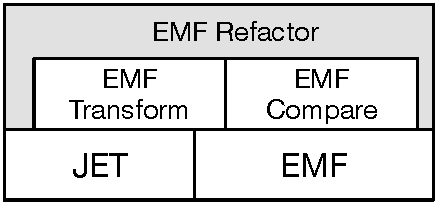
\includegraphics[scale=0.9]{images/EMFRefactorArchitecture}
	\fadaptada{hostesupporting}
\end{figure}


\begin{figure}[h]
	\centering
	% Requires \usepackage{graphicx}
	\caption{\textit{Wizard} para aplicar refatoração do EMF Refactor.}
	\label{fig:wizard_emfCOmpare}
	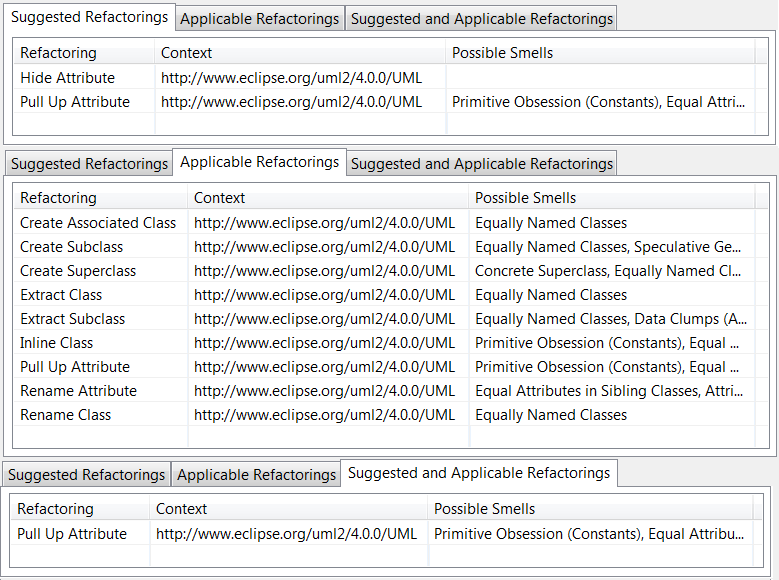
\includegraphics[scale=0.7]{images/EMFRefactorWizard}
	\fdireta{hostesupporting}
\end{figure}

Existem duas principais diferenças entre a KDM-RE e a ferramenta EMF Refactor. A primeira é que a ferramenta EMF Refactor não se preocupa em sincronizar as instâncias de um determino metamodelo após a aplicação das refatorações; diferentemente da KDM-Re, a qual define um módulo de sincronização exclusivo para essa característica. A segunda diferença está relacionada com a identificação de qual(is) refatoração(ões) aplicar. Por meio da EMF Refactor, é possível identificar quais refatorações precisam ser realizadas, ou seja, a ferramenta permite identificar quais são os \textit{bad smells}; KDM-RE no seu estado atual não permite a identificação de \textit{bad smells}.


\begin{figure}[h]
	\centering
	% Requires \usepackage{graphicx}
	\caption{Arquitetura da ferramenta Refactory.}
	\label{fig:refactory}
	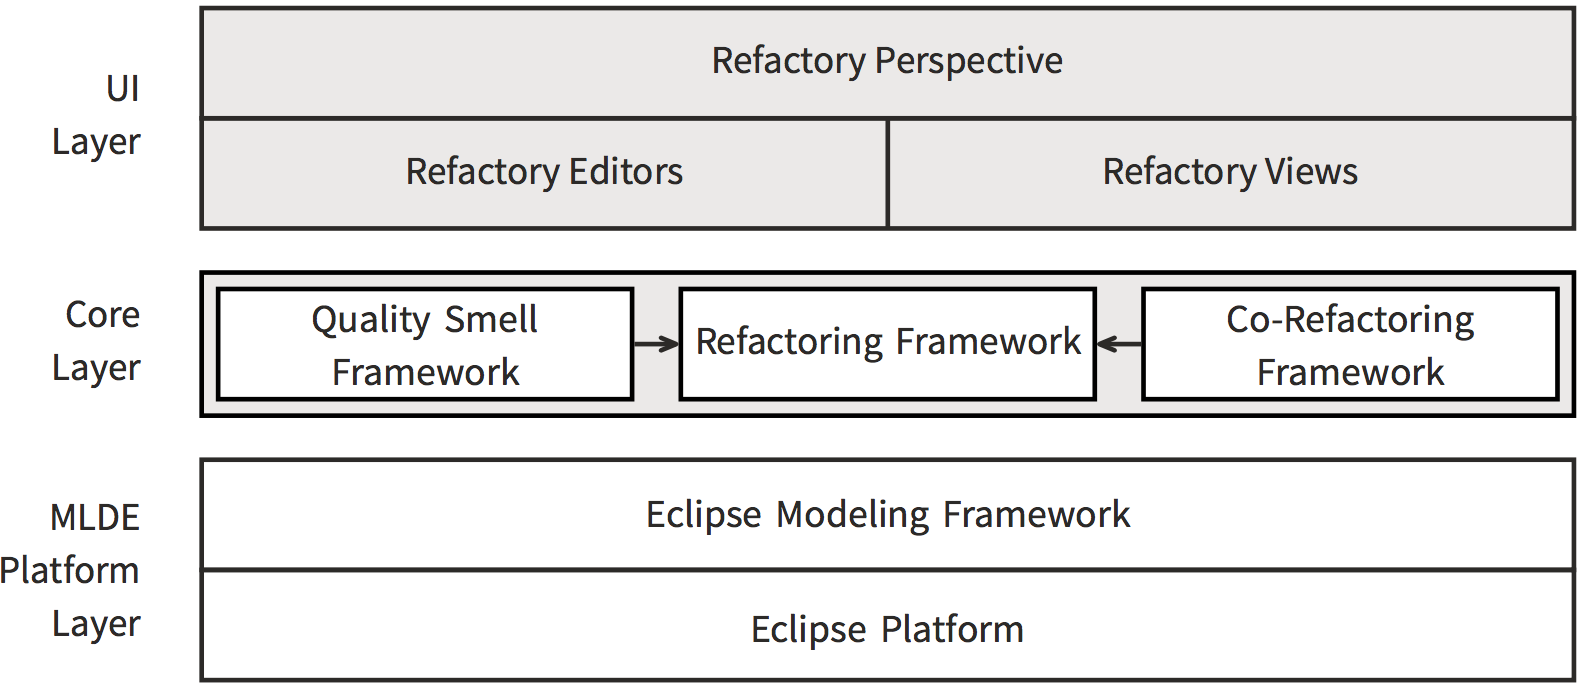
\includegraphics[scale=0.2]{images/refactoryArchitecture}
	\fdireta{Reimann_2015}
\end{figure}

Outra ferramenta relacionada a KDM-RE é a Refactory\footnote{\texttt{http://www.modelrefactoring.org/index.php/Refactoring}}. A arquitetura da ferramenta Refactory é apresentada na Figura~\ref{fig:refactory}. Da mesma forma que a KDM-RE, Refactory também contém três camadas: (\textit{i}) \textit{Platform Layer}, (\textit{ii}) \textit{Core Layer} e (\textit{iii}) \textit{UI layer}. A camada \textit{Core} contém três módulos: (\textit{i}) \textit{Quality Smell Framework}, (\textit{ii}) \textit{Refactoring Framework} e (\textit{iii}) \textit{Co-Refactoring Framework}. Note que, Refactory também é baseada no EMF e pode refatorar qualquer metamodelo definido pelo EMF. Além disso, de acordo com~\citeonline{reimann2010role}, Refactory, foi criada para permitir refatorações genéricas. Os autores afirmam que, realizar uma refatoração, por exemplo, \textit{extract method} em Java é o mesmo mecanismo para um sistema representado por instância da UML. As refatorações são todas implementas em QVT e as asserções são implementadas em OCL. Do mesmo modo que a KDM-RE, as refatorações da Refactory também são realizadas por meio de combinação de operações atômicas.




~\citeonline{mohamed2011m} propõem uma abordagem e uma ferramenta denominada M-Refactor. M-Refactor possui duas principais funcionalidades: (\textit{i}) identificar \textit{bad-smells} em instâncias do metamodelo UML e (\textit{ii}) aplicar refatorações em instâncias do metamodelo UML. A identificação dos \textit{bad-smells} é realizada em diagramas de classe e diagramas de sequência da UML. Os \textit{bad-smells} identificados são representados graficamente como apresentado na Figura~\ref{fig:m_refactor}. Após a identificação e visualização dos \textit{bad-smells}, o usuário pode aplicar as refatorações. Da mesma forma que a KDM-RE, M-Refactor também permite aplicar refatorações diretamente em diagramas de classe da UML. Porém, M-Refactor não se preocupa em sincronizar outras representações da UML como a KDM-RE.

\begin{figure}[h]
	\centering
	% Requires \usepackage{graphicx}
	\caption{Visão geral da ferramenta M-Refactor.}
	\label{fig:m_refactor}
	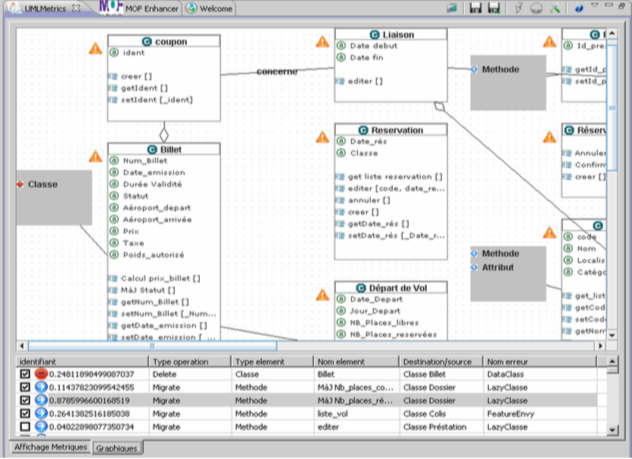
\includegraphics[scale=0.6]{images/m_refactor}
	\fdireta{mohamed2011m}
\end{figure}

\begin{figure}[h]
	\centering
	% Requires \usepackage{graphicx}
	\caption{Arquitetura da Ferramenta MOOSE.}
	\label{fig:moose}
	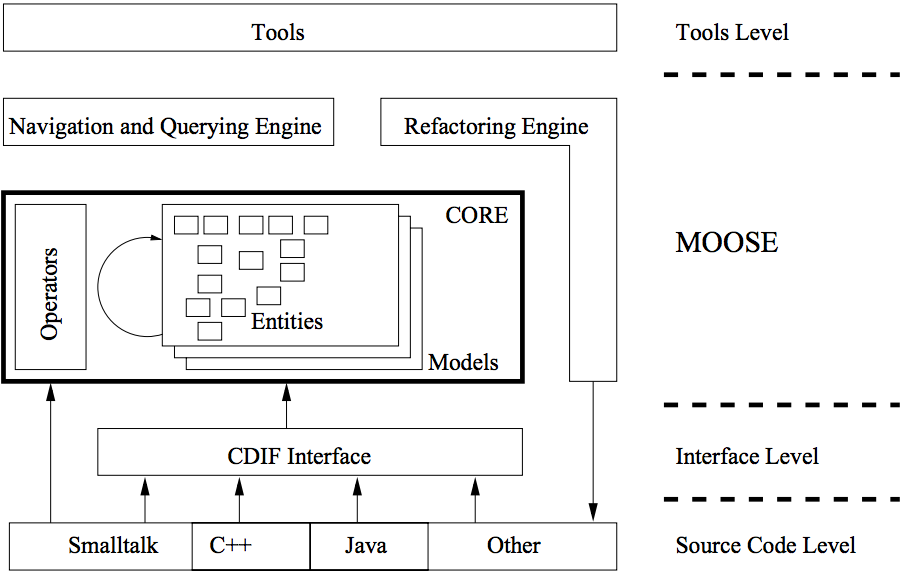
\includegraphics[scale=0.32]{images/MOOSEArchitecture}
	\fdireta{ducasse2000moose}
\end{figure}


Outra ferramenta relacionada é a MOOSE~\cite{tichelaar2000meta, ducasse2000moose}. A arquitetura da ferramenta MOOSE é apresentada na Figura~\ref{fig:moose}. Como pode ser observado, MOOSE aceita como entrada diversos tipos de linguagem de programação (Smalltalk, Java, C++, etc) e, em seguida, MOOSE transforma tais linguagens em um metamodelo denominado FAMIX~\cite{tichelaar2000meta}. Após realizar essa transformação, refatorações podem ser aplicadas. De acordo com os autores, MOOSE permite a aplicação de refatorações em nível de modelo de forma independente utilizando o metamodelo FAMIX~\cite{tichelaar2000meta}. MOOSE utiliza a ferramenta Refactoring Browser~\cite{roberts1997refactoring} e, assim, permite que as refatorações aplicadas em instâncias do metamodelo FAMIX sejam automaticamente replicas no código-fonte Smalltalk, porém, essa função apenas funciona quando a linguagem de entrada é a Smalltalk. Da mesma forma que a KDM-RE, MOOSE, permite a aplicação de refatorações de forma independente de linguagem - KDM-RE utiliza o metamodelo KDM e MOOSE utiliza o metamodelo FAMIX. Porém, MOOSE não busca sincronizar a instância do FAMIX após a realização de refatorações como a KDM-RE.

\begin{figure}[h]
	\centering
	% Requires \usepackage{graphicx}
	\caption{Visão geral da Ferramenta RACOoN.}
	\label{fig:racoon}
	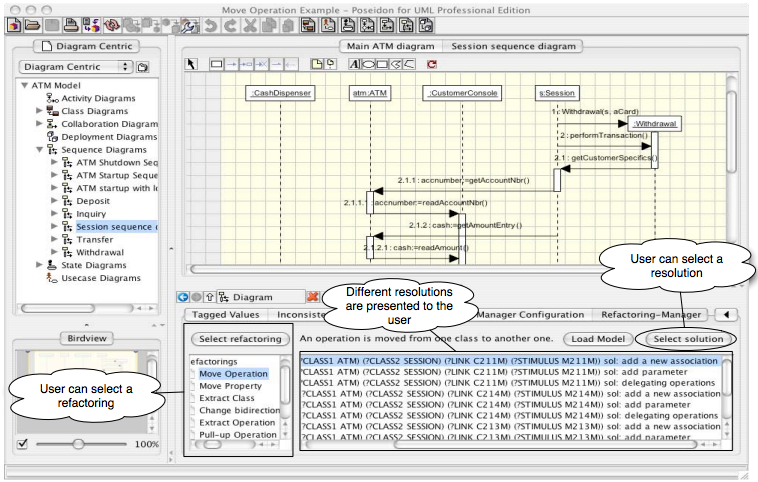
\includegraphics[scale=0.52]{images/fig_racoon}
	\fdireta{van2006model}
\end{figure}

RACOoN é um \textit{plug-in} desenvolvido por~\citeonline{van2006model}, ver Figura~\ref{fig:racoon}. Utilizando esse \textit{plug-in} regras de transformação em modelo podem ser implementadas, carregadas e em seguida serem executadas em diagramas da UML. RACOoN é uma ferramenta totalmente manual e permite que o usuário definida qual refatoração almeja aplicar, sendo de inteira responsabilidade do usuário definir a refatoração corretamente. Inconsistência encontradas durante a aplicação de múltiplas refatorações são apresentadas para o usuário juntamente com um conjunto de soluções. RACOoN e KDM-RE são similares, poém, RACOoN foi definida para diagramas da UML e KDM-RE para o metamodelo KDM.


~\citeonline{Boger_2003} definiram uma extensão da ferramenta Refactoring Browser~\cite{roberts1997refactoring} e criaram a primeira ferramenta para aplicar refatorações em modelos UML. Seguindo a mesma linha de pensamento,
VisTra~\cite{vstolc2010visual} é uma ferramenta visual desenvolvida também como um \textit{plug-in} para o ambiente de desenvolvimento Eclipse, a qual aplica refatorações em diagramas de classes da UML. Essa ferramenta permite que o usuário defina regras de transformação graficamente e, em seguida, a ferramenta gera automaticamente restrições em OCL e regras de transformações em QVT. Da mesma forma, NEPTUNE~\cite{millan2009ocl} é uma ferramenta que permite verificar e transformar instâncias do metamodelo UML. Essa ferramenta utiliza uma extensão da OCL denominada pOCL para automatizar a detecção de \textit{bad-smells}. Em seguida, NEPTUNE sugere um conjunto de refatorações para reparar os \textit{bad-smells} identificados. 

Embora todas as ferramentas identificadas apliquem refatorações em nível de modelo, nenhuma realiza as refatorações utilizando o metamodelo KDM. Além disso, nenhuma ferramenta identificada fornece uma forma para prover a reutilização de refatorações. Dessa forma, acredita-se que a KDM-RE é uma contribuição para a área de pesquisa de refatoração em nível de modelo. Além disso, somente a KDM-RE utiliza o metamodelo KDM como base para as refatorações, o que significa que a KDM-RE é independente de plataforma e linguagem de programação. Embora todas as ferramentas identificas utilizem o EMF e/ou UML, nenhuma utiliza o metamodelo KDM. Uma das vantagens de utilizar o KDM é que ele possui diversas metaclasses para representar níveis diferentes de um determinado sistema.

\section{Considerações Finais}\label{sec:consideracoes_final_kdm_re}

Este capítulo, apresenta a ferramenta KDM-RE. Essa ferramenta foi implementada, de modo a ser utilizada em conjunto com os demais recursos oferecidos pelo ambiente de desenvolvimento Eclipse IDE. Dessa forma, a KDM-RE foi desenvolvida utilizando os conceitos de \textit{plug-ins}. Três \textit{plug-ins} foram criados e são organizados em módulos de acordo com a sua predominante funcionalidade. Os três principais módulos da KDM-RE são: (\textit{i}) módulo de refatoração, (\textit{ii}) módulo do SRM e (\textit{iii}) módulo de sincronização. 

O primeiro módulo é responsável por criar uma infraestrutura que auxilia o engenheiro de software a aplicar refatorações em nível de modelos no contexto do metamodelo KDM. O engenheiro de software pode aplicar as refatorações no metamodelo KDM por meio de duas interfaces, a primeira denominada \textit{model browser} permite que o engenheiro tenha uma visão de árvore da instância do metamodelo KDM e aplique refatorações. A segunda interface permite que o engenheiro de software aplique refatorações diretamente em diagramas de classe da UML. Embora o engenheiro de software utilize diagrama de classe da UML na segunda interface as refatorações são aplicadas transparentemente na instância do metamodelo KDM - o diagrama de classe da UML é utilizado apenas para extrair metadados (nome da classe, nome do atributo, tipo do atributo, etc) que são enviadas como entrada para a refatoração pré-definida em ATL.

O segundo módulo é responsável por disponibilizar uma DSL para instanciar o metamodelo SRM apresentado no Capítulo~\ref{chapter:Toward_a_Refactoring_Metamodel_for_KDM}. Além disso o módulo do SRM fornece uma forma de reutilizar e compartilhar refatorações por meio de instâncias do metamodelo SRM. Esse segundo módulo converte a sintaxe e a semântica da DSL em um arquivo XMI. Cada marcação desse arquivo XMI representa uma instância da metaclasse do metamodelo SRM. Para permitir o reúso e compartilhamento de refatorações de forma consistente e abrangente um repositório remoto foi criado. Esse repositório remoto é dedicado para executar solicitações RESTful. Instâncias do metamodelo SRM são enviadas e recebidas por meio da API RESTful. JPA e o banco de dados MySQL foram utilizados para realizar as persistências das instâncias do metamodelo SRM.

Finalmente o terceiro módulo é responsável por implementar uma forma de manter a instância do metamodelo KDM sincronizada e consistente. Esse módulo tem como objetivo propagar e sincronizar uma determinada instância do metamodelo KDM após a aplicação de refatorações. Essas propagações são realizadas com base em regras pré-definidas e apresentadas no Apêndice~\ref{apendice:regras_propagacao}. Como o metamodelo KDM possui um conjunto de pacotes para representar diferentes artefatos é importante manter a instância e todos os outros artefatos sincronizados após a aplicação de refatorações. No Capítulo~\ref{chapter:avaliacao} um conjunto de avaliações são executadas para avaliar a abordagem apresentada nesta Tese.